\chapter{Sistemas de ecuaciones lineales}\label{sel}

En el capítulo anterior se estudiaron las matrices como arreglos ordenados de números y múltiples operaciones respecto a ellas junto a múltiples aplicaciones. En este capítulo se estudiarán los \textbf{sistemas de ecuaciones lineales}, una parte fundamental del álgebra lineal y de su fundamento básico: los espacios vectoriales.

En el capítulo \ref{vegern} se estudiaron los vectores como unidades con magnitud, dirección y sentido que son usados en múltiples ramas de la ciencia como física e ingenierías. Allí también se les dio sentido como vectores en coordenadas (Definición \ref{def:vectorescoordenadas}), por lo que podríamos pensar en vectores como una matriz fila $\mathbf{u}=(4,2,3)$ o como una matriz columna $\mathbf{u}=\begin{pmatrix}4\\2\\3\end{pmatrix}$. 

Piense ahora en el siguiente problema: dada una matriz $A=\begin{pmatrix}a_{11}&a_{12}&\cdots &a_{1n}\\a_{21}&a_{22}&\cdots &a_{2n}\\ \vdots&\vdots&\ddots &\vdots\\ a_{m1}&a_{m2}&\cdots &a_{mn}\end{pmatrix}$ de tamaño $m\times n$, si la multiplicamos por un vector $\mathbf{x}=\begin{pmatrix}x_1\\x_2\\\vdots\\ x_n \end{pmatrix} \in \mathbb{R}^n$, obtenemos el vector 
\begin{equation*}
A\mathbf{x} = \begin{pmatrix} a_{11}x_1+a_{12}x_2+\cdots + a_{1n}x_n\\a_{21}x_1+a_{22}x_2+\cdots + a_{2n}x_n\\\vdots \\ a_{m1}x_1+a_{m2}x_2+\cdots + a_{mn}x_n\end{pmatrix}.
\end{equation*}

Este vector $A\mathbf{x}$ será un vector que llamaremos combinación lineal de las columnas de $A$, cuyos coeficientes son las coordenadas de $\mathbf{x}$. Aunque en la Definición \ref{def:comblineal} se explicará este concepto de manera general, aquí podremos decir que para $\mathbb{R}^n$:

\begin{definition}[Combinación lineal de vectores en $\mathbb{R}^n$] 
Una \textbf{combinación lineal} de los vectores $\mathbf{v}_1,\mathbf{v}_2,\ldots, \mathbf{v}_k$ de $\mathbb{R}^n$ es un vector de la forma $m_1\mathbf{v}_1+m_2\mathbf{v}_2+\cdots + m_k\mathbf{v}_k$, donde $m_1, m_2,\ldots, m_k$ son escalares.
\end{definition} 

\begin{example} 
$\begin{pmatrix} 1&2&5\\0&1&3\\2&5&1 \end{pmatrix}\begin{pmatrix} 2\\5\\3 \end{pmatrix} = 2\begin{pmatrix}1\\0\\2 \end{pmatrix}+5\begin{pmatrix} 2\\1\\5\end{pmatrix}+3\begin{pmatrix} 5\\3\\1\end{pmatrix}= \begin{pmatrix} 2+10+15\\0+5+9\\4+25+3 \end{pmatrix}= \begin{pmatrix} 27\\14\\32 \end{pmatrix}.$
\end{example}

Por otro lado, observe que si $x_1,x_2,\dots, x_n$ son incógnitas, la ecuación $a_{11}x_1+a_{12}x_2+\dots + a_{1n}x_n=b_1$ es una ecuación lineal, pues las incógnitas tienen grado 1. Esto nos lleva a definir un sistema de ecuaciones lineales:

\begin{definition}[Sistema de ecuaciones lineales]
Un sistema de $m$ ecuaciones lineales con $n$ incógnitas es un arreglo expresado por

$\begin{cases}
a_{11}x_1 + a_{12}x_2 + \cdots + a_{1n}x_n &= b_1  \\
a_{21}x_1 + a_{22}x_2 + \cdots + a_{2n}x_n &= b_2  \\
&\vdots \\\
a_{m1}x_1 + a_{m2}x_2 + \cdots + a_{mn}x_n &= b_m,
\end{cases}$

que puede ser representado en forma matricial por $A\mathbf{x} = \mathbf{b}$
siendo
\begin{equation*}
A = \begin{bmatrix}
a_{11} & a_{12} & \cdots & a_{1n} \\
a_{21} & a_{22} & \cdots & a_{2n} \\
\vdots & \vdots & \ddots & \vdots \\
a_{m1} & a_{m2} & \cdots & a_{mn}
\end{bmatrix}, \quad
\mathbf{x} = \begin{bmatrix}
x_1 \\ x_2 \\ \vdots \\ x_n
\end{bmatrix} \quad \text{y} \quad
\mathbf{b} = \begin{bmatrix}
b_1 \\ b_2 \\ \vdots \\ b_m
\end{bmatrix},
\end{equation*}
respectivamente, la matriz de coeficientes, el vector de incógnitas y el vector de términos independientes.
\end{definition}

\begin{definition}[Tipos de soluciones de un sistema lineal]
Encontrar la \textbf{solución} o el conjunto-solución o, aún, la solución general de un sistema de ecuaciones significa hallar todos los valores de $\mathbf{x} \in \mathbb{R}^n$ que resuelven simultáneamente las ecuaciones.
En el caso de sistemas lineales con coeficientes reales, las posibilidades son tres:
\begin{enumerate}
\item El sistema posee una única solución.
\item El sistema posee infinitas soluciones.
\item El sistema no posee solución.
\end{enumerate}
En los dos primeros casos, el sistema es \textbf{consistente} o \textbf{compatible}; en el último, es \textbf{inconsistente} o \textbf{incompatible}.
\end{definition}

Se demostrará que un sistema de ecuaciones lineales $A\mathbf{x} = \mathbf{b}$ con $n$ incógnitas posee soluciones si y solo si el rango de la matriz aumentada $[A|\mathbf{b}]$ es igual al rango de la matriz de coeficientes $A$ (recuerde la Definición \ref{def:rango}). Si además $\text{rank}(A) = n$, entonces la solución es única. En caso contrario, existen infinitas soluciones reales (o complejas).

Los sistemas de ecuaciones lineales se dividen básicamente en dos tipos, homogéneos y no homogéneos. Se proporciona la definición a continuación:

\begin{definition}[Sistema de ecuaciones lineales homogéneo]
Un \textbf{sistema de ecuaciones lineales homogéneo} es un sistema de $m$ ecuaciones lineales con $n$ incógnitas de la forma

$\begin{cases}
a_{11}x_1 + a_{12}x_2 + \cdots + a_{1n}x_n &= 0 \nonumber\\
a_{21}x_1 + a_{22}x_2 + \cdots + a_{2n}x_n &= 0 \nonumber\\
&\vdots \\
a_{m1}x_1 + a_{m2}x_2 + \cdots + a_{mn}x_n &= 0,
\end{cases}$

donde todos los términos independientes son iguales a cero.

En forma matricial, se expresa como $A\mathbf{x} = \mathbf{0},$
donde $A$ es la matriz de coeficientes de tamaño $m \times n$, $\mathbf{x}$ es el vector de incógnitas y $\mathbf{0}$ es el vector nulo de $\mathbb{R}^m$.
\end{definition}

En general, se demostrará en el Teorema \ref{thm:carsisthom} que la suma de dos soluciones de un sistema homogéneo es solución y si se multiplica una solución por un escalar también lo es.

Encontrar las soluciones de un sistema de ecuaciones es un trabajo que se ha venido resolviendo desde el bachillerato; tal vez recuerde los métodos de sustitución, reducción o igualación, o tal vez también la regla de Cramer. Nuestra idea aquí no es reducirnos a sistemas $2\times 2$ o $3\times 3$, sino más bien generar métodos para miles de incógnitas y ecuaciones. El método que usaremos más a menudo será el \textbf{método de eliminación gaussiana}, creado por el príncipe de las matemáticas Carl Friedrich Gauss. Nosotros ya estamos habituados a él (Lema \ref{lem:gauss}) o en su versión del método de Gauss-Jordan (Lema \ref{lem:gauss-jordan}).


\begin{example}[Sistema $2 \times 2$ - Intersección de rectas]
Consideremos el siguiente sistema de ecuaciones lineales:
$\begin{cases}
2x + 3y &= 7 \\
x - y &= 1
\end{cases}$
\begin{myproof} Resolviendo por el método de Gauss-Jordan (Lema \ref{lem:gauss-jordan}), la matriz aumentada del sistema es:
$$\left[\begin{array}{cc|c}
2 & 3 & 7 \\
1 & -1 & 1
\end{array}\right]$$

\textbf{Paso 1:} $f_1\leftrightarrow f_2$ (pivote más conveniente) $\left(\begin{array}{cc|c}
1 & -1 & 1 \\
2 & 3 & 7
\end{array}\right),$

\textbf{Paso 2:} $f_2 - 2f_1 \rightarrow f_2$ $\left(\begin{array}{cc|c}
1 & -1 & 1 \\
0 & 5 & 5
\end{array}\right),$

\textbf{Paso 3:} $\frac{1}{5}f_2 \rightarrow f_2$: $\left(\begin{array}{cc|c}
1 & -1 & 1 \\
0 & 1 & 1
\end{array}\right),$

\textbf{Paso 4:} $f_1 + f_2 \rightarrow f_1$: $\left(\begin{array}{cc|c}
1 & 0 & 2 \\
0 & 1 & 1
\end{array}\right)$

Por lo tanto: $x = 2$ e $y = 1$, es decir, la solución es $(2, 1)$.

\textbf{Interpretación geométrica:}
Cada ecuación lineal en dos variables representa una recta en el plano cartesiano, por lo cual las ecuaciones $2x + 3y = 7$ y $x - y = 1$ son rectas y $(2, 1)$ corresponde a su \textbf{punto de intersección}. Este es el único punto que satisface simultáneamente ambas ecuaciones.

\begin{figure}[H]
\centering
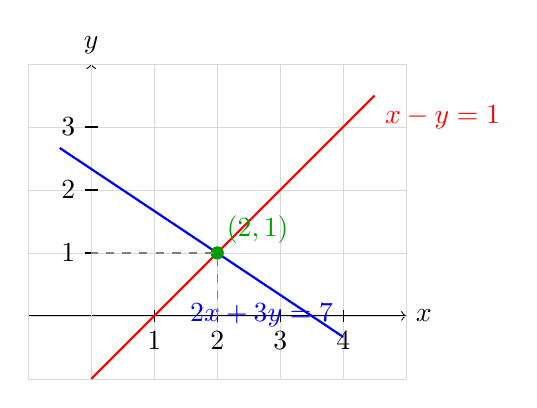
\begin{tikzpicture}[scale=0.8]
    % Configuración de los ejes
    \draw[->] (-1,0) -- (5,0) node[right] {$x$};
    \draw[->] (0,-1) -- (0,4) node[above] {$y$};
    
    % Grilla
    \draw[help lines, color=gray!30] (-1,-1) grid (5,4);
    
    % Etiquetas de los ejes
    \foreach \x in {1,2,3,4}
        \draw (\x,0.1) -- (\x,-0.1) node[below] {$\x$};
    \foreach \y in {1,2,3}
        \draw (0.1,\y) -- (-0.1,\y) node[left] {$\y$};
    
    % Primera recta: 2x + 3y = 7, despejamos y = (7-2x)/3
    \draw[blue, thick, domain=-0.5:4] plot (\x, {(7-2*\x)/3}) 
        node[above left] {$2x + 3y = 7$};
    
    % Segunda recta: x - y = 1, despejamos y = x - 1
    \draw[red, thick, domain=0:4.5] plot (\x, {\x-1}) 
        node[below right] {$x - y = 1$};
    
    % Punto de intersección
    \fill[green!60!black] (2,1) circle (3pt);
    \node[green!60!black, above right] at (2,1) {$(2,1)$};
    
    % Líneas punteadas hasta los ejes
    \draw[dashed, gray] (2,0) -- (2,1) -- (0,1);
\end{tikzpicture}
\caption{Intersección de las rectas $2x + 3y = 7$ y $x - y = 1$. La solución del sistema corresponde al punto donde ambas rectas se cruzan.}
\label{fig:sistema2x2}
\end{figure}
\end{myproof}
\end{example}

\begin{rem} Es importante notar que los planos son la \textbf{generalización tridimensional} de las rectas. Mientras que una ecuación lineal con dos incógnitas $ax + by = c$ representa una recta en el plano, una ecuación lineal con tres incógnitas $ax + by + cz = d$ representa un plano en el espacio.
\end{rem}

\begin{example}[Sistema $3 \times 3$ - Intersección de planos]
Calcule la solución del siguiente sistema de ecuaciones lineales $\begin{cases}
x + 2y + z &= 9 \\
2x - y + 2z &= 8 \\
x + y - z &= 1
\end{cases}:$

\begin{myproof} La matriz aumentada del sistema es:
$\left(\begin{array}{ccc|c}
1 & 2 & 1 & 9 \\
2 & -1 & 2 & 8 \\
1 & 1 & -1 & 1
\end{array}\right).$ Usaremos el método de Gauss-Jordan (Lema \ref{lem:gauss-jordan}).

\textbf{Paso 1:} $f_2 - 2f_1 \rightarrow f_2$ y $f_3 - f_1 \rightarrow f_3$:
$\left(\begin{array}{ccc|c}
1 & 2 & 1 & 9 \\
0 & -5 & 0 & -10 \\
0 & -1 & -2 & -8
\end{array}\right)$

\textbf{Paso 2:} $-\frac{1}{5}f_2 \rightarrow f_2$: $\left(\begin{array}{ccc|c}
1 & 2 & 1 & 9 \\
0 & 1 & 0 & 2 \\
0 & -1 & -2 & -8
\end{array}\right)$

\textbf{Paso 3:} $f_3 + f_2 \rightarrow f_3$: $\left(\begin{array}{ccc|c}
1 & 2 & 1 & 9 \\
0 & 1 & 0 & 2 \\
0 & 0 & -2 & -6
\end{array}\right)$

\textbf{Paso 4:} $-\frac{1}{2}f_3 \rightarrow f_3$: $\left(\begin{array}{ccc|c}
1 & 2 & 1 & 9 \\
0 & 1 & 0 & 2 \\
0 & 0 & 1 & 3
\end{array}\right)$

\textbf{Paso 5:}  $f_1 - f_3 \rightarrow f_1$: $\left(\begin{array}{ccc|c}
1 & 2 & 0 & 6 \\
0 & 1 & 0 & 2 \\
0 & 0 & 1 & 3
\end{array}\right)$

\textbf{Paso 6:} $f_1 - 2f_2 \rightarrow f_1$: $\left(\begin{array}{ccc|c}
1 & 0 & 0 & 2 \\
0 & 1 & 0 & 2 \\
0 & 0 & 1 & 3
\end{array}\right)$

Por lo tanto: $x = 2$, $y = 2$ y $z = 3$, es decir, la solución es $(2, 2, 3)$.

\textbf{Interpretación geométrica:}
Cada ecuación lineal en tres variables representa un \textbf{plano} en el espacio tridimensional, por lo que la solución del sistema $(2, 2, 3)$ corresponde al \textbf{punto de intersección común} de estos tres planos. Este es el único punto en el espacio que pertenece simultáneamente a los tres planos, es decir, que satisface las tres ecuaciones al mismo tiempo.

\begin{figure}[H]
\centering
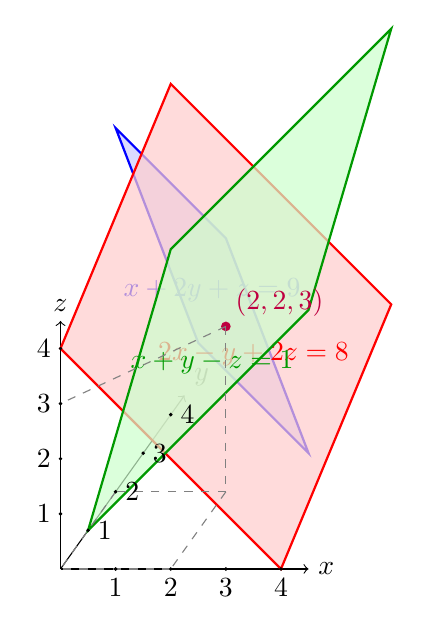
\begin{tikzpicture}[scale=0.7, 
    x={(1cm,0cm)}, y={(0.5cm,0.7cm)}, z={(0cm,1cm)}]
    
    % Ejes de coordenadas
    \draw[->] (0,0,0) -- (4.5,0,0) node[right] {$x$};
    \draw[->] (0,0,0) -- (0,4.5,0) node[above right] {$y$};
    \draw[->] (0,0,0) -- (0,0,4.5) node[above] {$z$};
    
    % Primer plano: x + 2y + z = 9 (azul)
    % Definimos algunos puntos del plano
    \coordinate (A1) at (1,0,8);
    \coordinate (A2) at (3,0,6);
    \coordinate (A3) at (1,3,2);
    \coordinate (A4) at (3,3,0);
    
    \fill[blue!20, opacity=0.7] (A1) -- (A2) -- (A4) -- (A3) -- cycle;
    \draw[blue, thick] (A1) -- (A2) -- (A4) -- (A3) -- cycle;
    \node[blue] at (2,1.5,4) {$x + 2y + z = 9$};
    
    % Segundo plano: 2x - y + 2z = 8 (rojo)
    \coordinate (B1) at (0,0,4);
    \coordinate (B2) at (4,0,0);
    \coordinate (B3) at (0,4,6);
    \coordinate (B4) at (4,4,2);
    
    \fill[red!20, opacity=0.7] (B1) -- (B2) -- (B4) -- (B3) -- cycle;
    \draw[red, thick] (B1) -- (B2) -- (B4) -- (B3) -- cycle;
    \node[red] at (2.5,2,2.5) {$2x - y + 2z = 8$};
    
    % Tercer plano: x + y - z = 1 (verde)
    \coordinate (C1) at (0,1,0);
    \coordinate (C2) at (4,1,4);
    \coordinate (C3) at (0,4,3);
    \coordinate (C4) at (4,4,7);
    
    \fill[green!20, opacity=0.7] (C1) -- (C2) -- (C4) -- (C3) -- cycle;
    \draw[green!60!black, thick] (C1) -- (C2) -- (C4) -- (C3) -- cycle;
    \node[green!60!black] at (1.5,2.5,2) {$x + y - z = 1$};
    
    % Punto de intersección
    \fill[purple] (2,2,3) circle (2.5pt);
    \node[purple, above right] at (2,2,3) {$(2,2,3)$};
    
    % Líneas punteadas desde el punto a los ejes
    \draw[dashed, gray] (2,2,3) -- (2,2,0);
    \draw[dashed, gray] (2,2,0) -- (2,0,0);
    \draw[dashed, gray] (2,2,0) -- (0,2,0);
    \draw[dashed, gray] (2,0,0) -- (0,0,0);
    \draw[dashed, gray] (0,2,0) -- (0,0,0);
    \draw[dashed, gray] (2,2,3) -- (0,0,3);
    
    % Etiquetas en los ejes
    \foreach \x in {1,2,3,4}
        \draw (\x,0,0) node[below] {$\x$};
    \foreach \y in {1,2,3,4}
        \draw (0,\y,0) node[right] {$\y$};
    \foreach \z in {1,2,3,4}
        \draw (0,0,\z) node[left] {$\z$};
        
    % Puntos de referencia en los ejes
    \foreach \x in {1,2,3,4}
        \fill (\x,0,0) circle (1pt);
    \foreach \y in {1,2,3,4}
        \fill (0,\y,0) circle (1pt);
    \foreach \z in {1,2,3,4}
        \fill (0,0,\z) circle (1pt);
\end{tikzpicture}
\caption{Intersección de tres planos en el espacio. Cada ecuación lineal con tres incógnitas representa un plano, y la solución del sistema corresponde al punto donde los tres planos se intersectan.}
\label{fig:sistema3x3}
\end{figure}
\end{myproof}
\end{example}

\begin{rem} En general, un sistema de $n$ ecuaciones lineales con $n$ incógnitas que tiene solución única corresponde geométricamente a la intersección de $n$ hiperplanos en $\mathbb{R}^n$. Para $n = 2$ tenemos rectas (hiperplanos de dimensión 1 en $\mathbb{R}^2$), para $n = 3$ tenemos planos (hiperplanos de dimensión 2 en $\mathbb{R}^3$), y así sucesivamente. Para \textbf{sistemas $2 \times 2$:}

\begin{figure}[H]
\centering
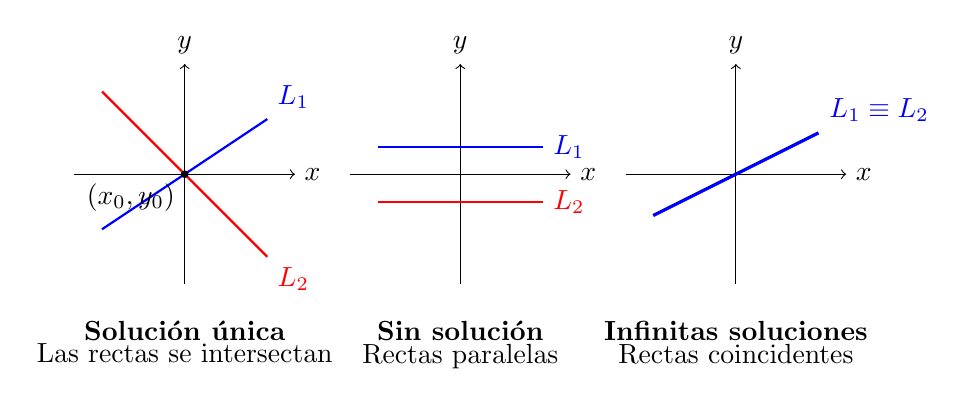
\begin{tikzpicture}[scale=0.7]
    % Caso 1: Solución única
    \begin{scope}[xshift=-5cm]
        \draw[->] (-2,0) -- (2,0) node[right] {$x$};
        \draw[->] (0,-2) -- (0,2) node[above] {$y$};
        \draw[blue, thick] (-1.5,-1) -- (1.5,1) node[above right] {$L_1$};
        \draw[red, thick] (-1.5,1.5) -- (1.5,-1.5) node[below right] {$L_2$};
        \fill[black] (0,0) circle (2pt);
        \node[below left] at (0,0) {$(x_0, y_0)$};
        \node[below] at (0,-2.5) {\textbf{Solución única}};
        \node[below] at (0,-2.9) {Las rectas se intersectan};
    \end{scope}
    
    % Caso 2: Sin solución
    \begin{scope}
        \draw[->] (-2,0) -- (2,0) node[right] {$x$};
        \draw[->] (0,-2) -- (0,2) node[above] {$y$};
        \draw[blue, thick] (-1.5,0.5) -- (1.5,0.5) node[right] {$L_1$};
        \draw[red, thick] (-1.5,-0.5) -- (1.5,-0.5) node[right] {$L_2$};
        \node[below] at (0,-2.5) {\textbf{Sin solución}};
        \node[below] at (0,-2.9) {Rectas paralelas};
    \end{scope}
    
    % Caso 3: Infinitas soluciones
    \begin{scope}[xshift=5cm]
        \draw[->] (-2,0) -- (2,0) node[right] {$x$};
        \draw[->] (0,-2) -- (0,2) node[above] {$y$};
        \draw[blue, very thick] (-1.5,-0.75) -- (1.5,0.75) node[above right] {$L_1 \equiv L_2$};
        \node[below] at (0,-2.5) {\textbf{Infinitas soluciones}};
        \node[below] at (0,-2.9) {Rectas coincidentes};
    \end{scope}
\end{tikzpicture}
\caption{Interpretación geométrica de sistemas $2 \times 2$}
\end{figure}

\vspace{0.5cm}

\textbf{Casos para sistemas $3 \times 3$:}

De manera análoga, para sistemas de $3$ ecuaciones con $3$ incógnitas, tenemos tres planos en $\mathbb{R}^3$:

\begin{itemize}
    \item \textbf{Solución única:} Los tres planos se intersectan en un único punto.
    \item \textbf{Sin solución:} Los planos no tienen intersección común (por ejemplo, tres planos paralelos distintos, o dos planos paralelos y un tercero que los corta).
    \item \textbf{Infinitas soluciones:} Los tres planos se intersectan en una recta (intersección común es una línea) o los tres planos son coincidentes (intersección común es todo el plano).
\end{itemize}

En general, para un sistema $n \times n$:
\begin{itemize}
    \item La \textbf{solución única} corresponde a que los $n$ hiperplanos se intersecten en exactamente un punto de $\mathbb{R}^n$.
    \item \textbf{Sin solución} ocurre cuando no existe intersección común de todos los hiperplanos.
    \item \textbf{Infinitas soluciones} se presenta cuando la intersección común tiene más de un punto (puede ser una línea, un plano, etc., dependiendo de la dimensión).
\end{itemize}
\end{rem}
\begin{rem}
Al aplicar el método de eliminación gaussiana a un sistema de ecuaciones lineales $Ax = b$, el comportamiento del sistema puede determinarse mediante el análisis de la matriz aumentada $(A|b)$ en su forma escalonada:

\begin{itemize}
    \item \textbf{Sistema inconsistente (sin solución):} El sistema no tiene solución si y solo si existe una fila en la forma escalonada de $(A|b)$ de la forma $(0, 0, \ldots, 0 | c)$ donde $c \neq 0$. Esto corresponde a una ecuación de la forma $0 = c$ con $c \neq 0$, la cual es imposible de satisfacer.
    
    \item \textbf{Sistema con infinitas soluciones:} Si el sistema es consistente y el número de filas no nulas en la forma escalonada de la matriz de coeficientes $A$ es menor que el número de incógnitas, entonces el sistema tiene infinitas soluciones. En este caso, aparecerán filas de la forma $(0, 0, \ldots, 0 | 0)$ en la matriz aumentada, y habrá variables libres que pueden tomar cualquier valor real.
    
    \item \textbf{Sistema con solución única:} Si el sistema es consistente y el número de filas no nulas en la forma escalonada de $A$ es igual al número de incógnitas, entonces el sistema tiene una única solución.
\end{itemize}
\end{rem}

\begin{definition}[Variables básicas y libres]
En el contexto de un sistema de ecuaciones lineales $A\mathbf{x}=\mathbf{b}$, consideremos la forma escalonada obtenida mediante eliminación gaussiana. Las variables del sistema se clasifican en dos categorías:

\begin{itemize}
\item \textbf{Variables básicas}: Son aquellas variables que corresponden a las columnas que contienen los elementos pivote en la forma escalonada de la matriz aumentada del sistema.

\item \textbf{Variables libres} (o \textbf{parámetros}): Son las variables restantes, es decir, aquellas que corresponden a columnas sin elemento pivote en la forma escalonada.
\end{itemize}

Esta clasificación es fundamental para expresar la solución general del sistema en forma paramétrica, donde las variables libres actúan como parámetros independientes que determinan el conjunto completo de soluciones.
\end{definition}

\begin{example} Dado el sistema de ecuaciones $\begin{cases}
x_1+x_2+x_3+x_4=0\\
2x_1+2x_2+x_3+x_4=0\\
x_1+x_2-x_3+x_4=0
\end{cases}$ 

Use el método de eliminación gaussiana para calcular sus soluciones. Determine las variables libres correspondientes y encuentre las ecuaciones paramétricas de la solución: 

\begin{myproof} La matriz aumentada del sistema es 
$\left(\begin{array}{cccc|c}
1 & 1 & 1 & 1 & 0 \\
2 & 2 & 1 & 1 & 0 \\
1 & 1 & -1 & 1 & 0
\end{array}\right).$ Aplicando eliminación gaussiana:

\textbf{Paso 1:} $f_2 - 2f_1\ \to f_2$ y $f_3 - f_1\to f_3$: $\left(\begin{array}{cccc|c}
1 & 1 & 1 & 1 & 0 \\
0 & 0 & -1 & -1 & 0 \\
0 & 0 & -2 & 0 & 0
\end{array}\right)$

\textbf{Paso 2:} Como la segunda columna no tiene pivote, se busca pivote en la tercera columna. Se toma $-2$ como pivote en la fila 3. $f_3 - 2f_2\to f_3$
$\left(\begin{array}{cccc|c}
\boxed{1} & 1 & 1 & 1 & 0 \\
0 & 0 & \boxed{-1} & -1 & 0 \\
0 & 0 & 0 & \boxed{2} & 0
\end{array}\right)$

De esta matriz se tiene que $x_1, x_3, x_4$ son columnas con pivotes  $1$, $-2$, $2$ (variables básicas) y $x_2$ es la variable libre (columna sin pivote).

La \textbf{Solución paramétrica} se toma a partir de la forma escalonada en el sistema equivalente:
\begin{align*}
x_1 + x_2 + x_3 + x_4 &= 0 \quad (1)\\
-x_3 - x_4 &= 0 \quad (2)\\
2x_4 &= 0 \quad (3)
\end{align*}

Resolviendo por sustitución hacia atrás: 
\begin{itemize}
\item De la ecuación (3): $x_4 = 0$
\item De la ecuación (2): $-x_3 - 0 = 0 \Rightarrow x_3 = 0$
\item De la ecuación (1): $x_1 + x_2 + 0 + 0 = 0 \Rightarrow x_1 = -x_2$
\end{itemize}

Sea $x_2 = t$ donde $t \in \mathbb{R}$ es el parámetro libre. 

Entonces la solución paramétrica es:

$\begin{pmatrix}
x_1 \\ x_2 \\ x_3 \\ x_4
\end{pmatrix} = \begin{pmatrix}
-t \\ t \\ 0 \\ 0
\end{pmatrix} = t\begin{pmatrix}
-1 \\ 1 \\ 0 \\ 0
\end{pmatrix}, \quad t \in \mathbb{R}.$

Por lo tanto, el conjunto solución es una recta que pasa por el origen en la dirección del vector $(-1, 1, 0, 0)$.
\end{myproof}
\end{example}

\begin{theorem}[Teorema de Rouché-Frobenius]
Sea $A$ una matriz de $m \times n$ y $b$ un vector de $\mathbb{R}^m$. Consideremos el sistema de ecuaciones lineales $Ax = b$. Sea $\tilde{A} = [A|b]$ la matriz ampliada del sistema. Entonces:
\begin{enumerate}
    \item El sistema $Ax = b$ tiene solución si y solo si $\text{rango}(A) = \text{rango}(\tilde{A})$.
    \item Si el sistema tiene solución, entonces:
    \begin{itemize}
        \item Si $\text{rango}(A) = n$, la solución es única.
        \item Si $\text{rango}(A) < n$, el sistema tiene infinitas soluciones que dependen de $n - \text{rango}(A)$ parámetros libres.
    \end{itemize}
\end{enumerate}
\end{theorem}

\begin{proof}
Demostraremos cada parte del teorema usando eliminación gaussiana.

\textbf{Parte 1:} El sistema $Ax = b$ tiene solución si y solo si $\text{rango}(A) = \text{rango}(\tilde{A})$. Mediante operaciones elementales de fila, podemos transformar la matriz ampliada $\tilde{A} = [A|b]$ a su forma escalonada reducida. Las operaciones elementales de fila no cambian el conjunto de soluciones del sistema.

$(\Rightarrow)$ Supongamos que el sistema $Ax = b$ tiene solución. Al aplicar eliminación gaussiana a $\tilde{A}$, nunca obtendremos una fila de la forma $[0 \, 0 \, \cdots \, 0 \, | \, c]$ con $c \neq 0$, pues esto correspondería a la ecuación $0 = c$, que es una contradicción. Por tanto, el número de filas no nulas en la forma escalonada de $A$ es igual al número de filas no nulas en la forma escalonada de $\tilde{A}$, es decir, $\text{rango}(A) = \text{rango}(\tilde{A})$.

$(\Leftarrow)$ Supongamos que $\text{rango}(A) = \text{rango}(\tilde{A})$. Esto significa que al reducir $\tilde{A}$ por filas, no aparece ninguna fila de la forma $[0 \, 0 \, \cdots \, 0 \, | \, c]$ con $c \neq 0$. Por tanto, el sistema escalonado equivalente es consistente y tiene al menos una solución.

\textbf{Parte 2:} Si el sistema tiene solución, sea $r = \text{rango}(A)$ el número de filas no nulas en la forma escalonada de $A$.

Si $r = n$, entonces en la forma escalonada reducida tenemos $n$ variables pivote (una en cada columna de $A$). Esto significa que cada variable está determinada de manera única, por lo que la solución es única.

Si $r < n$, entonces hay $r$ variables pivote y $n - r$ variables libres. Las variables libres pueden tomar cualquier valor, y las variables pivote se expresan en términos de estas variables libres. Por tanto, el sistema tiene infinitas soluciones que dependen de $n - r$ parámetros libres.
\end{proof}

\begin{example}
Consideremos el sistema de ecuaciones lineales:
$\begin{cases}
x_1 + 2x_2 + x_3 &= 4\\
2x_1 + 4x_2 + 3x_3 &= 9\\
x_1 + 2x_2 + 2x_3 &= 6
\end{cases}$

Aplicaremos el teorema de Rouché-Frobenius para determinar si el sistema tiene solución y, en caso afirmativo, clasificar el tipo de solución.
\end{example}

\begin{myproof} Primero, escribimos la matriz de coeficientes $A$ y la matriz ampliada $\tilde{A}$:
$$A = \begin{pmatrix}
1 & 2 & 1\\
2 & 4 & 3\\
1 & 2 & 2
\end{pmatrix}, \quad \tilde{A} = \begin{pmatrix}
1 & 2 & 1 & 4\\
2 & 4 & 3 & 9\\
1 & 2 & 2 & 6
\end{pmatrix}$$

Calculamos el rango de $A$ mediante eliminación gaussiana:

$A = \begin{pmatrix}
1 & 2 & 1\\
2 & 4 & 3\\
1 & 2 & 2
\end{pmatrix} \xrightarrow{\begin{array}{c}f_2 - 2f_1 \to f_2\\ f_3 - f_1 \to f_3\end{array}} \begin{pmatrix}
1 & 2 & 1\\
0 & 0 & 1\\
0 & 0 & 1
\end{pmatrix} \xrightarrow{f_3 - f_2 \to f_3} \begin{pmatrix}
1 & 2 & 1\\
0 & 0 & 1\\
0 & 0 & 0
\end{pmatrix}$ 

Por tanto, $\text{rango}(A) = 2$.

Ahora calculamos el rango de $\tilde{A}$:
$\tilde{A} = \begin{pmatrix}
1 & 2 & 1 & 4\\
2 & 4 & 3 & 9\\
1 & 2 & 2 & 6
\end{pmatrix} \xrightarrow{\begin{array}{c}f_2 - 2f_1 \to f_2\\ f_3 - f_1 \to f_3\end{array}} \begin{pmatrix}
1 & 2 & 1 & 4\\
0 & 0 & 1 & 1\\
0 & 0 & 1 & 2
\end{pmatrix} \xrightarrow{f_3 - f_2 \to f_3} \begin{pmatrix}
1 & 2 & 1 & 4\\
0 & 0 & 1 & 1\\
0 & 0 & 0 & 1
\end{pmatrix}$

Por tanto, $\text{rango}(\tilde{A}) = 3$.

\textbf{Conclusión:} Como $\text{rango}(A) = 2 \neq 3 = \text{rango}(\tilde{A})$, el teorema de Rouché-Frobenius nos dice que el sistema \textbf{no tiene solución}. La última fila de la matriz ampliada escalonada corresponde a la ecuación $0 = 1$, que es una contradicción, confirmando que el sistema es inconsistente.
\end{myproof}

\begin{rem} 
Un sistema de ecuaciones lineales $A\mathbf{x}=\mathbf{b}$ puede tener solución única, infinitas soluciones o ninguna solución. Para solución única es necesario (pero no suficiente) que $A$ sea cuadrada. Cuando $A$ es cuadrada e invertible, se garantiza existencia y unicidad de la solución para cualquier $mathbf{b}$, lo que permite extender el teorema de caracterización de matrices invertibles con propiedades de sistemas lineales.
\end{rem}

\begin{theorem}[Caracterización de matrices invertibles - Versión 3]\label{thm:invertible-equiv-v3}
Sea $A$ una matriz cuadrada de orden $n \times n$. Las siguientes afirmaciones son equivalentes:
\begin{enumerate}
    \item $A$ es invertible.
    \item La forma escalonada reducida de $A$ es la matriz identidad $I_n$.
    \item $A$ se puede escribir como producto de matrices elementales.
    \item $A$ tiene rango máximo ($\text{rango}(A) = n$).
    \item $\det(A) \neq 0$.
    \item $A\mathbf{x}=\mathbf{0}$ tiene únicamente la solución nula.
    \item $A\mathbf{x}=\mathbf{b}$ es consistente para cualquier vector $\mathbf{b}$.
    \item $A\mathbf{x}=\mathbf{b}$ tiene solución única para cualquier vector $\mathbf{b}$.
\end{enumerate}
\end{theorem}

\begin{proof}
Ya hemos demostrado la equivalencia de las afirmaciones (1)-(5) en versiones anteriores de este teorema. Procederemos a demostrar que estas son equivalentes a las afirmaciones (6)-(8).

\textbf{$(1) \Rightarrow (6)$:}
Supongamos que $A$ es invertible y sea $\mathbf{x}$ una solución de $A\mathbf{x}=\mathbf{0}$. Multiplicando ambos lados por $A^{-1}$ a la izquierda:
$$A^{-1}(A\mathbf{x}) = A^{-1}\mathbf{0}$$
$$(A^{-1}A)\mathbf{x} = \mathbf{0}$$
$$I_n\mathbf{x} = \mathbf{0}$$
$$\mathbf{x} = \mathbf{0}$$
Por lo tanto, la única solución del sistema homogéneo es la solución nula.

\textbf{$(6) \Rightarrow (4)$:}
Supongamos que $A\mathbf{x}=\mathbf{0}$ tiene únicamente la solución nula. Consideremos la forma escalonada reducida de $A$, llamémosla $R$. Sabemos que existe una matriz invertible $P$ (producto de matrices elementales) tal que $PA = R$.

El sistema $A\mathbf{x}=\mathbf{0}$ es equivalente al sistema $R\mathbf{x}=\mathbf{0}$ (tienen las mismas soluciones). Como $A\mathbf{x}=\mathbf{0}$ tiene únicamente la solución nula, entonces $R\mathbf{x}=\mathbf{0}$ también tiene únicamente la solución nula.

Si $R$ tuviera una fila de ceros, digamos la fila $k$, entonces las variables correspondientes a las columnas sin pivote serían variables libres, lo que implicaría que el sistema $R\mathbf{x}=\mathbf{0}$ tendría infinitas soluciones (contradicción). Por lo tanto, $R$ no puede tener filas de ceros.

Como $R$ es una matriz $n \times n$ en forma escalonada reducida sin filas de ceros, debe tener $n$ pivotes, uno en cada fila. Esto significa que $\text{rango}(A) = \text{rango}(R) = n$.

\textbf{$(1) \Rightarrow (7)$:}
Supongamos que $A$ es invertible. Para cualquier vector $\mathbf{b} \in \mathbb{R}^n$, consideremos el sistema $A\mathbf{x}=\mathbf{b}$. Como $A$ es invertible, podemos definir $\mathbf{x} = A^{-1}\mathbf{b}$. Verificamos que esta es efectivamente una solución:
$$A\mathbf{x} = A(A^{-1}\mathbf{b}) = (AA^{-1})\mathbf{b} = I_n\mathbf{b} = \mathbf{b}$$
Por lo tanto, el sistema es consistente para cualquier $\mathbf{b}$.

\textbf{$(7) \Rightarrow (4)$:}
Supongamos que $A\mathbf{x}=\mathbf{b}$ es consistente para cualquier vector $\mathbf{b}$. En particular, debe ser consistente para cada uno de los vectores canónicos $\mathbf{e}_1, \mathbf{e}_2, \ldots, \mathbf{e}_n$.

Consideremos la forma escalonada reducida de la matriz aumentada $(A|\mathbf{e}_i)$ para cada $i = 1, 2, \ldots, n$. Como cada sistema es consistente, ninguna de estas matrices aumentadas puede tener una fila de la forma $(0 \, 0 \, \cdots \, 0 \, | \, 1)$.

Esto significa que cuando reducimos la matriz $A$ a su forma escalonada, no puede aparecer una fila de ceros, pues de lo contrario algún sistema $A\mathbf{x}=\mathbf{e}_i$ sería inconsistente. Por lo tanto, la forma escalonada reducida de $A$ tiene $n$ pivotes, lo que implica que $\text{rango}(A) = n$.

\textbf{$(1) \Rightarrow (8)$:}
Supongamos que $A$ es invertible. Por la demostración anterior, sabemos que para cualquier $\mathbf{b}$, el sistema $A\mathbf{x}=\mathbf{b}$ tiene al menos una solución $\mathbf{x} = A^{-1}\mathbf{b}$. Para demostrar unicidad, supongamos que $\mathbf{x}_1$ y $\mathbf{x}_2$ son dos soluciones del sistema. Entonces:
$$A\mathbf{x}_1 = \mathbf{b} \quad \text{y} \quad A\mathbf{x}_2 = \mathbf{b}$$
Restando estas ecuaciones: $A(\mathbf{x}_1 - \mathbf{x}_2) = \mathbf{0}$. Por la afirmación (6), esto implica que $\mathbf{x}_1 - \mathbf{x}_2 = \mathbf{0}$, es decir, $\mathbf{x}_1 = \mathbf{x}_2$. Por lo tanto, la solución es única.

\textbf{$(8) \Rightarrow (6)$:}
Supongamos que $A\mathbf{x}=\mathbf{b}$ tiene solución única para cualquier vector $\mathbf{b}$. En particular, para $\mathbf{b} = \mathbf{0}$, el sistema $A\mathbf{x}=\mathbf{0}$ tiene solución única. Como sabemos que $\mathbf{x} = \mathbf{0}$ es siempre una solución del sistema homogéneo, esta debe ser la única solución.

Hemos demostrado el ciclo de implicaciones:
$$(1) \Rightarrow (6) \Rightarrow (4) \Rightarrow (1)$$
$$(1) \Rightarrow (7) \Rightarrow (4) \Rightarrow (1)$$  
$$(1) \Rightarrow (8) \Rightarrow (6) \Rightarrow (4) \Rightarrow (1)$$

Como ya habíamos establecido que (1)-(5) son equivalentes (Teorema \ref{thm:invertible-equiv-v2}), concluimos que todas las afirmaciones (1)-(8) son equivalentes.
\end{proof}

\begin{theorem}[Propiedades de los sistemas homogéneos] 
Dado un sistema de ecuaciones lineales homogéneo $A\mathbf{x}=\mathbf{0}$ se cumple:
\begin{enumerate}
\item Todo sistema homogéneo es \textbf{consistente}, pues siempre admite al menos la \textbf{solución trivial} $\mathbf{x} = \mathbf{0}$.
\item Si el sistema homogéneo tiene una solución no trivial, entonces tiene infinitas soluciones.
\item Un sistema homogéneo $A\mathbf{x} = \mathbf{0}$ con $n$ incógnitas tiene solución única (la trivial) si y solo si $\text{rank}(A) = n$.
\item Si $\text{rank}(A) < n$, entonces el sistema tiene infinitas soluciones no triviales.
\end{enumerate}
\end{theorem}

\begin{proof} 

\textbf{Propiedad 1:} Sea $A\mathbf{x} = \mathbf{0}$ un sistema homogéneo. Sustituyendo $\mathbf{x} = \mathbf{0},$ $A\mathbf{0} = \mathbf{0}$ y esta igualdad es siempre verdadera, independientemente de la matriz $A$. Por tanto, $\mathbf{x} = \mathbf{0}$ es siempre una solución, y el sistema es consistente.


\textbf{Propiedad 2:} Supongamos que $\mathbf{x}_0 \neq \mathbf{0}$ es una solución no trivial de $A\mathbf{x} = \mathbf{0}$, es decir, $A\mathbf{x}_0 = \mathbf{0}$.

Para cualquier escalar $k \in \mathbb{R}$, consideremos $\mathbf{x} = k\mathbf{x}_0$:
$$A(k\mathbf{x}_0) = k(A\mathbf{x}_0) = k\mathbf{0} = \mathbf{0}$$

Por tanto, $k\mathbf{x}_0$ es solución para todo $k \in \mathbb{R}$. Como hay infinitos valores de $k$, existen infinitas soluciones.

\textbf{Propiedad 3:} Distinguimos dos casos según si $A$ es cuadrada o no.

\textbf{Caso 1:} Si $A$ es una matriz cuadrada $n \times n$:

Por el Teorema de Caracterización de Matrices Invertibles (equivalencias 4 y 6):
$$\text{rank}(A) = n \iff A\mathbf{x} = \mathbf{0} \text{ tiene únicamente la solución nula}$$

\textbf{Caso 2:} Si $A$ es una matriz $m \times n$ con $m \neq n$:

El rango de $A$ satisface $\text{rank}(A) \leq \min(m,n)$.

Utilizaremos el teorema del rango-nulidad: para cualquier matriz $A$ de tamaño $m \times n$,
$\text{rank}(A) + \text{nullity}(A) = n$
donde $\text{nullity}(A) = \dim(\text{Nul}(A))$ es la dimensión del espacio nulo de $A$.

\begin{itemize}
\item Si $\text{rank}(A) = n$, entonces $\text{nullity}(A) = n - n = 0$. Esto significa que $\dim(\text{Nul}(A)) = 0$, por lo que el espacio nulo contiene únicamente el vector cero. Por tanto, $A\mathbf{x} = \mathbf{0}$ tiene únicamente la solución trivial $\mathbf{x} = \mathbf{0}$.

\item Si $\text{rank}(A) < n$, entonces $\text{nullity}(A) = n - \text{rank}(A) > 0$. Esto significa que $\dim(\text{Nul}(A)) > 0$, por lo que el espacio nulo contiene vectores no nulos. Por tanto, el sistema $A\mathbf{x} = \mathbf{0}$ tiene soluciones no triviales.
\end{itemize}


\textbf{Propiedad 4:} Si $\text{rank}(A) < n$, entonces por la Propiedad 3, el sistema $A\mathbf{x} = \mathbf{0}$ no tiene solución única. Como sabemos por la Propiedad 1 que siempre tiene al menos la solución trivial, debe tener más de una solución.

Si existe una solución no trivial $\mathbf{x}_0$, entonces por la Propiedad 2, existen infinitas soluciones.

Para mostrar que efectivamente existe una solución no trivial, consideremos la forma escalonada reducida $R$ de la matriz $A$. Como $\text{rank}(A) < n$, la matriz $R$ tiene menos de $n$ pivotes, digamos $r = \text{rank}(A) < n$.

Esto significa que hay $n - r > 0$ variables libres en el sistema $R\mathbf{x} = \mathbf{0}$.

Podemos construir una solución no trivial asignando el valor 1 a una de las variables libres y 0 a las demás variables libres. Las variables básicas quedan determinadas por los valores de las variables libres a través de las ecuaciones del sistema.

Como al menos una variable (la variable libre elegida) tiene valor 1, la solución obtenida es no trivial.
\end{proof}

\begin{theorem}[Regla de Cramer]
Sea $A$ una matriz cuadrada de orden $n \times n$ con $\det(A) \neq 0$, y sea $\mathbf{b}$ un vector en $\mathbb{R}^n$. Entonces el sistema de ecuaciones lineales $A\mathbf{x} = \mathbf{b}$ tiene una única solución dada por:
$x_i = \frac{\det(A_i)}{\det(A)}, \quad i = 1, 2, \ldots, n$
donde $A_i$ es la matriz obtenida al reemplazar la $i$-ésima columna de $A$ por el vector $\mathbf{b}$.
\end{theorem}

\begin{proof}
Como $\det(A) \neq 0$, la matriz $A$ es invertible por el teorema de caracterización de matrices invertibles (Teorema \ref{thm:invertible-equiv-v3}). Por lo tanto, el sistema $A\mathbf{x} = \mathbf{b}$ tiene una única solución $\mathbf{x} = A^{-1}\mathbf{b}$.

Recordemos que la matriz inversa puede expresarse como:
$A^{-1} = \frac{1}{\det(A)}\text{adj}(A)$
donde $\text{adj}(A)$ es la matriz adjunta (o adjunta clásica) de $A$, cuyas entradas son:
$[\text{adj}(A)]_{ij} = (-1)^{j+i}M_{ji}$
siendo $M_{ji}$ el menor obtenido al eliminar la fila $j$ y la columna $i$ de $A$.

La solución del sistema es:
$\mathbf{x} = A^{-1}\mathbf{b} = \frac{1}{\det(A)}\text{adj}(A)\mathbf{b}$

Para encontrar la $i$-ésima componente $x_i$ de la solución, calculamos el producto de la $i$-ésima fila de $\text{adj}(A)$ con el vector $\mathbf{b}$:
$x_i = \frac{1}{\det(A)}\sum_{j=1}^{n} [\text{adj}(A)]_{ij}b_j = \frac{1}{\det(A)}\sum_{j=1}^{n} (-1)^{i+j}M_{ji}b_j$

Ahora, consideremos la matriz $A_i$ obtenida al reemplazar la $i$-ésima columna de $A$ por el vector $\mathbf{b}$:
$A_i = \begin{pmatrix}
a_{11} & \cdots & a_{1,i-1} & b_1 & a_{1,i+1} & \cdots & a_{1n} \\
a_{21} & \cdots & a_{2,i-1} & b_2 & a_{2,i+1} & \cdots & a_{2n} \\
\vdots & \ddots & \vdots & \vdots & \vdots & \ddots & \vdots \\
a_{n1} & \cdots & a_{n,i-1} & b_n & a_{n,i+1} & \cdots & a_{nn}
\end{pmatrix}$

Al expandir $\det(A_i)$ por la $i$-ésima columna (que contiene los elementos de $\mathbf{b}$), obtenemos:
$\det(A_i) = \sum_{j=1}^{n} b_j \cdot (-1)^{j+i} \cdot M'_{ji}$

donde $M'_{ji}$ es el menor obtenido al eliminar la fila $j$ y la columna $i$ de $A_i$. 

Observemos que este menor $M'_{ji}$ es exactamente igual al menor $M_{ji}$ de la matriz original $A$, ya que al eliminar la fila $j$ y la columna $i$ de $A_i$, eliminamos precisamente la fila $j$ y la columna $i$ que contenía el elemento $b_j$, quedando la misma submatriz que se obtiene al eliminar la fila $j$ y la columna $i$ de $A$.

Por lo tanto:
$\det(A_i) = \sum_{j=1}^{n} b_j \cdot (-1)^{j+i} \cdot M_{ji} = \sum_{j=1}^{n} (-1)^{i+j}M_{ji}b_j$

Comparando con la expresión que obtuvimos para $x_i$:
$x_i = \frac{1}{\det(A)}\sum_{j=1}^{n} (-1)^{i+j}M_{ji}b_j = \frac{\det(A_i)}{\det(A)}$

Esto completa la demostración de la Regla de Cramer.
\end{proof}

\begin{prob} Tres especies de ardillas han sido llevadas a una isla con una población inicial total de 2.000. Después de 10 años, la especie I ha duplicado su población y la especie II ha incrementado su población en un 50\%, mientras que la especie III se ha extinguido. Si el incremento en la población de la especie I es igual que el de la especie II y si la población total se ha incrementado en 500, determine la población inicial de las tres especies.

\begin{myproof}
Definamos $x_1$, $x_2$ y $x_3$ como las poblaciones iniciales de las tres especies de ardillas. De las condiciones del problema:
\begin{itemize}
    \item Población inicial total: $x_1 + x_2 + x_3 = 2000$
    \item Población final total: $2x_1 + \frac{3}{2}x_2 + 0 = 2500$ (ya que la especie III se extinguió)
    \item El incremento de la especie I es igual al incremento de la especie II, así el Incremento de I es $2x_1 - x_1 = x_1$ mientras que el Incremento de II es $\frac{3}{2}x_2 - x_2 = \frac{1}{2}x_2.$ Por tanto: $x_1 = \frac{1}{2}x_2.$
\end{itemize}

Esto nos lleva al siguiente sistema de ecuaciones \(
\left\{
\begin{array}{rcl}
x_1 + x_2 + x_3 &=& 2000\\
2x_1 + \frac{3}{2}x_2 &=& 2500\\
x_1 - \frac{1}{2}x_2 &=& 0
\end{array}
\right.
\)

Usando la regla de Cramer. La matriz de coeficientes del sistema es:


\(
A = \begin{pmatrix}
1 & 1 & 1\\
2 & \frac{3}{2} & 0\\
1 & -\frac{1}{2} & 0
\end{pmatrix}
\)  y $\det A = -\frac{5}{2}.$

Para encontrar $x_1$: \(
A_1 = \begin{pmatrix}
2000 & 1 & 1\\
2500 & \frac{3}{2} & 0\\
0 & -\frac{1}{2} & 0
\end{pmatrix}
\), así \( \det A_1 = -1250 .\)

Para encontrar $x_2$: \(
A_2 = \begin{pmatrix}
1 & 2000 & 1\\
2 & 2500 & 0\\
1 & 0 & 0
\end{pmatrix}
,\) así \( \det A_2 = -2500 \)

Para encontrar $x_3$: \(
A_3 = \begin{pmatrix}
1 & 1 & 2000\\
2 & \frac{3}{2} & 2500\\
1 & -\frac{1}{2} & 0
\end{pmatrix}
\) y \(
\det A_3 = -1250 \)

De esta manera: $\begin{cases}
x_1 &= \frac{\det A_1}{\det A} = \frac{-1250}{-\frac{5}{2}} = \frac{1250 \cdot 2}{5} = 500\\
x_2 &= \frac{\det A_2}{\det A} = \frac{-2500}{-\frac{5}{2}} = \frac{2500 \cdot 2}{5} = 1000\\
x_3 &= \frac{\det A_3}{\det A} = \frac{-1250}{-\frac{5}{2}} = \frac{1250 \cdot 2}{5} = 500
\end{cases}$

Por tanto, las poblaciones iniciales son: 500 ardillas de la especie I, 1000 ardillas de la especie II y 500 ardillas de la especie III.
\end{myproof}
\end{prob}


\begin{prob} 
Utilice eliminación gaussiana o de Gauss-Jordan para resolver los sistemas de ecuaciones lineales. Si existe solución única, indíquela; si hay infinitas soluciones, identifique las variables libres y exprese el conjunto solución en forma paramétrica; si no hay solución, explique claramente la razón mediante la forma escalonada o inconsistencia detectada.

    \begin{enumerate}[$a)$]
    \item  $\left\lbrace \begin{array}{ccc}
2x-y+2z&=&-4\\
6x-3y+6z&=&-12\\
-4x+2y-4z&=&8\\
\end{array} \right. $ 
    
    \begin{myproof}
    Matriz aumentada y operaciones:
    \[
    \begin{pmatrix}
    2 & -1 & 2 & | & -4 \\
    6 & -3 & 6 & | & -12 \\
    -4 & 2 & -4 & | & 8 \\
    \end{pmatrix}
    \]
    
    \begin{align*}
    &f_2 - 3f_1\to f_2 \\
    &\begin{pmatrix}
    2 & -1 & 2 & | & -4 \\
    0 & 0 & 0 & | & 0 \\
    -4 & 2 & -4 & | & 8 \\
    \end{pmatrix} \\
    &f_3 + 2f_1\to f_3: \\
    &\begin{pmatrix}
    2 & -1 & 2 & | & -4 \\
    0 & 0 & 0 & | & 0 \\
    0 & 0 & 0 & | & 0 \\
    \end{pmatrix}
    \end{align*}
    
    \textbf{Análisis:} 
    \begin{itemize}
    \item Sistema equivalente: $2x - y + 2z = -4$.
    \item Variables libres: $y$ y $z$.
    \end{itemize}
    
    \textbf{Solución paramétrica:}
    \[
    \begin{pmatrix} x \\ y \\ z \end{pmatrix} = 
    \begin{pmatrix} \frac{y}{2} - z - 2 \\ y \\ z \end{pmatrix} = 
    y \begin{pmatrix} \frac{1}{2} \\ 1 \\ 0 \end{pmatrix} + 
    z \begin{pmatrix} -1 \\ 0 \\ 1 \end{pmatrix} + 
    \begin{pmatrix} -2 \\ 0 \\ 0 \end{pmatrix}, \quad y,z \in \mathbb{R}.
    \]
    \end{myproof}

 \item  $\left\lbrace \begin{array}{ccc}
x_1+2x_2-x_3&=&4\\
3x_1+4x_2-2x_3&=&7\\
\end{array} \right. $ 
    
    \begin{myproof}
    Matriz aumentada y operaciones:
    \[
    \begin{pmatrix}
    1 & 2 & -1 & | & 4 \\
    3 & 4 & -2 & | & 7 \\
    \end{pmatrix}
    \]
    
    \begin{align*}
    &f_2 - 3f_1 \to f_2: \\
    &\begin{pmatrix}
    1 & 2 & -1 & | & 4 \\
    0 & -2 & 1 & | & -5 \\
    \end{pmatrix} \\
    &-\frac{1}{2}f_2\to f_2: \\
    &\begin{pmatrix}
    1 & 2 & -1 & | & 4 \\
    0 & 1 & -\frac{1}{2} & | & \frac{5}{2} \\
    \end{pmatrix} \\
    &f_1 - 2f_2\to f_1: \\
    &\begin{pmatrix}
    1 & 0 & 0 & | & -1 \\
    0 & 1 & -\frac{1}{2} & | & \frac{5}{2} \\
    \end{pmatrix}
    \end{align*}
    
    \textbf{Solución paramétrica:}
    \[
    \begin{pmatrix} x_1 \\ x_2 \\ x_3 \end{pmatrix} = 
    \begin{pmatrix} -1 \\ \frac{5}{2} \\ 0 \end{pmatrix} + 
    x_3 \begin{pmatrix} 0 \\ \frac{1}{2} \\ 1 \end{pmatrix}, \quad x_3 \in \mathbb{R}.
    \]
    \end{myproof}

 \item $ \left\lbrace\begin{array}{ccc}
x+2y-2z&=&b_1\\
2x+5y-4z&=&b_2\\
4x+9y-8z&=&b_3\\
\end{array} \right.  $ 
    
    \begin{myproof}
    Matriz aumentada:
    \[
    \begin{pmatrix}
    1 & 2 & -2 & | & b_1 \\
    2 & 5 & -4 & | & b_2 \\
    4 & 9 & -8 & | & b_3 \\
    \end{pmatrix}
    \]
    
    \textbf{Forma escalonada:}
    \[
    \begin{pmatrix}
    1 & 2 & -2 & | & b_1 \\
    0 & 1 & 0 & | & b_2 - 2b_1 \\
    0 & 0 & 0 & | & b_3 - b_2 - 2b_1 \\
    \end{pmatrix}
    \]
    
    \textbf{Análisis:} 
    \begin{itemize}
    \item Si $b_3 - b_2 - 2b_1 \neq 0$: sistema inconsistente.
    \item Si $b_3 - b_2 - 2b_1 = 0$: infinitas soluciones con variable libre $z$.
    \end{itemize}
    
    \textbf{Solución paramétrica (cuando existe):}
    \[
    \begin{pmatrix} x \\ y \\ z \end{pmatrix} = 
    \begin{pmatrix} 5b_1 - 2b_2 \\ b_2 - 2b_1 \\ 0 \end{pmatrix} + 
    z \begin{pmatrix} 2 \\ 0 \\ 1 \end{pmatrix}, \quad z \in \mathbb{R}.
    \]
    \end{myproof}
	
	\item $\left\lbrace \begin{array}{ccc}
	2x_2+x_3+x_4&=&1\\
	2x_1+4x_2+4x_3+2x_4+2x_5&=&1\\
	3x_1+6x_2+6x_3&=&1\\
	2x_2+x_3+2x_4+4x_5&=&0\\
	\end{array} \right. $ 
	
	\begin{myproof}
    Matriz aumentada (reordenada):
    \[
    \begin{pmatrix}
    2 & 4 & 4 & 2 & 2 & | & 1 \\
    0 & 2 & 1 & 1 & 0 & | & 1 \\
    3 & 6 & 6 & 0 & 0 & | & 1 \\
    0 & 2 & 1 & 2 & 4 & | & 0 \\
    \end{pmatrix}
    \]
    
    \textbf{Forma escalonada reducida:}
    \[
    \begin{pmatrix}
    1 & 2 & 2 & 1 & 1 & | & \frac{1}{2} \\
    0 & 2 & 1 & 1 & 0 & | & 1 \\
    0 & 0 & 0 & 1 & 4 & | & -1 \\
    0 & 0 & 0 & 0 & 9 & | & -\frac{7}{2} \\
    \end{pmatrix}
    \]
    
    \textbf{Solución:}
    \begin{align*}
    &x_5 = -\frac{7}{18} \\
    &x_4 = -1 - 4\left(-\frac{7}{18}\right) = \frac{5}{9} \\
    &2x_2 + x_3 = 1 - \frac{5}{9} = \frac{4}{9} \quad \text{(variable libre } x_3\text{)} \\
    &x_1 = \frac{1}{2} - 2x_2 - 2x_3 - x_4 - x_5 = -\frac{1}{9} - x_3
    \end{align*}
    
    \textbf{Solución paramétrica:}
    \[
    \begin{pmatrix} x_1 \\ x_2 \\ x_3 \\ x_4 \\ x_5 \end{pmatrix} = 
    \begin{pmatrix} -\frac{1}{9} \\ \frac{2}{9} \\ 0 \\ \frac{5}{9} \\ -\frac{7}{18} \end{pmatrix} + 
    x_3 \begin{pmatrix} -1 \\ -\frac{1}{2} \\ 1 \\ 0 \\ 0 \end{pmatrix}, \quad x_3 \in \mathbb{R}.
    \]
    \end{myproof}
    \end{enumerate}
\end{prob}

\begin{prob} 
Determine los valores del parámetro \( t \) para los cuales el siguiente sistema tiene solución única, infinitas soluciones o ninguna solución. Justifique mediante análisis de rango y consistencia.

\[
\left\lbrace  
\begin{array}{rcl}
x_1 + x_2 + x_3 &=& 4 \\
x_3 &=& 2 \\
\left(t^2 - 4\right)x_3 &=& t + 2 \\
\end{array} 
\right. 
\]

\begin{myproof}
Aplicamos eliminación gaussiana a la matriz aumentada: \(
\begin{pmatrix}
1 & 1 & 1 & | & 4 \\
0 & 0 & 1 & | & 2 \\
0 & 0 & t^2-4 & | & t+2 \\
\end{pmatrix}
\)

\( f_3 - (t^2-4) \cdot f_2 \to f_3 \): \(
\begin{pmatrix}
1 & 1 & 1 & | & 4 \\
0 & 0 & 1 & | & 2 \\
0 & 0 & 0 & | & -2t^2 + t + 10 \\
\end{pmatrix}.
\)

\begin{itemize}
\item \textbf{Rango y consistencia:} 
  \begin{itemize}
  \item \(\text{rango}(A) = 2\) (dos filas no nulas en forma escalonada)
  \item \(\text{rango}(\tilde{A}) = 2\) si \(-2t^2 + t + 10 = 0\), y \(3\) en otro caso.
  \end{itemize}

\item \textbf{Solución única:} Imposible. La segunda columna no tiene pivote, lo que implica una variable libre (\(x_2\)) si el sistema es consistente.

\item \textbf{Infinitas soluciones:} Ocurre cuando \(\text{rango}(A) = \text{rango}(\tilde{A}) = 2\). Esto requiere:
  \[
  -2t^2 + t + 10 = 0 \implies t = \frac{1 \pm \sqrt{1 + 80}}{4} = \frac{1 \pm 9}{4}
  \]
  Así, \( t = \dfrac{5}{2} \) o \( t = -2 \). En estos casos, \(x_2\) es variable libre y las soluciones son de la forma:
  \[
  \begin{pmatrix} x_1 \\ x_2 \\ x_3 \end{pmatrix} = \begin{pmatrix} 2 - x_2 \\ x_2 \\ 2 \end{pmatrix}, \quad x_2 \in \mathbb{R}.
  \]

\item \textbf{Ninguna solución:} Ocurre cuando \(\text{rango}(A) = 2 \neq 3 = \text{rango}(\tilde{A})\), es decir, para \(t \neq \dfrac{5}{2}\) y \(t \neq -2\). La última ecuación sería \(0 = -2t^2 + t + 10 \neq 0\), una inconsistencia.
\end{itemize}
\end{myproof}
\end{prob}

\begin{prob} 
Dado el sistema de ecuaciones lineales

$\left\lbrace \begin{array}{ccccccc}
2x&-&y&+&2z&=&-4\\
6x&-&y&+&6z&=&-12\\
\end{array} \right. $

\begin{enumerate}[$a)$]
\item Añada una tercera ecuación para que el sistema tenga solución única.
\item Añada una tercera ecuación para que el sistema tenga soluciones infinitas.
\item Añada una tercera ecuación para que no tenga solución.
\end{enumerate}

\begin{myproof} \textbf{En general este problema puede tener múltiples soluciones, se muestran algunas posibilidades.}

\textbf{Solución del sistema original:} Aplicamos eliminación gaussiana:
\[
\begin{pmatrix}
2 & -1 & 2 & | & -4 \\
6 & -1 & 6 & | & -12 \\
\end{pmatrix}
\xrightarrow{f_2 - 3f_1\to f_2}
\begin{pmatrix}
2 & -1 & 2 & | & -4 \\
0 & 2 & 0 & | & 0 \\
\end{pmatrix}
\]
El sistema equivalente es:
\[
\left\lbrace \begin{array}{rcrcrcl}
2x & - & y & + & 2z & = & -4 \\
& & 2y & & & = & 0 \\
\end{array} \right.
\]
De la segunda ecuación: $y = 0$. Sustituyendo en la primera:
$2x + 2z = -4 \implies x + z = -2$.\\
La solución general es:
\[
(x, y, z) = (-2 - z,  0,  z) \quad \text{con} \quad z \in \mathbb{R}.
\]

\begin{enumerate}[$a)$]
\item \textbf{Solución única:} Añadir $z = 0$.\\
Justificación: Fija el valor de la variable libre ($z$). El sistema ampliado:
\[
\left\lbrace \begin{array}{rcrcrcl}
2x & - & y & + & 2z & = & -4 \\
6x & - & y & + & 6z & = & -12 \\
& & & & z & = & 0 \\
\end{array} \right.
\]
tiene solución única $(x, y, z) = (-2, 0, 0)$.

\item \textbf{Infinitas soluciones:} Añadir $x + z = -2$.\\
Justificación: Es consistente con la solución general (es combinación lineal de las ecuaciones originales). El sistema ampliado:
\[
\left\lbrace \begin{array}{rcrcrcl}
2x & - & y & + & 2z & = & -4 \\
6x & - & y & + & 6z & = & -12 \\
x & & & + & z & = & -2 \\
\end{array} \right.
\]
mantiene la solución general con $z$ libre.

\item \textbf{Ninguna solución:} Añadir $y = 1$.\\
Justificación: Contradice $y = 0$ de la solución general. El sistema ampliado:
\[
\left\lbrace \begin{array}{rcrcrcl}
2x & - & y & + & 2z & = & -4 \\
6x & - & y & + & 6z & = & -12 \\
& & y & & & = & 1 \\
\end{array} \right.
\]
es inconsistente (la tercera ecuación fuerza $y=1$, pero las primeras implican $y=0$).
\end{enumerate}
\end{myproof}
\end{prob}

\begin{prob} La curva $y=ax^2+bx+c$ que se observa en la figura \ref{parabolainterpolacion} pasa por los puntos $(x_1,y_1)$, $(x_2,y_2)$ y $(x_3,y_3)$.

\begin{multicols}{2}


\begin{enumerate}[a)]
\item Demuestre que los coeficientes $a$, $b$ y $c$ son soluciones del sistema cuya matriz aumentada es 
\[ \left( \begin{array}{ccc|c} 
x_1^2 & x_1 & 1 & y_1\\
x_2^2 & x_2 & 1 & y_2\\
x_3^2 & x_3 & 1 & y_3
\end{array} \right) \]

\item Use lo anterior para calcular el polinomio que pasa por los puntos $(1,3)$, $(2,5)$ y $(-1,9)$.
\end{enumerate}

\begin{figure}[H]
\centering
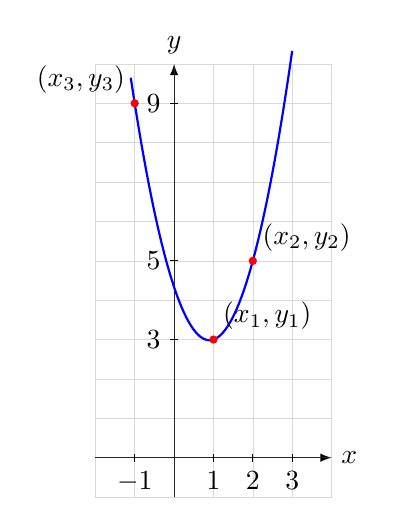
\begin{tikzpicture}[scale=0.5]
    % Ejes coordenados
    \draw[-latex] (-2,0) -- (4,0) node[right] {$x$};
    \draw[-latex] (0,-1) -- (0,10) node[above] {$y$};
    
    % Grilla opcional (comentar si no se desea)
    \draw[help lines, opacity=0.3] (-2,-1) grid (4,10);
    
    % Parábola: y = (5/3)x² - 3x + 13/3
    \draw[thick, blue, smooth, samples=100, domain=-1.1:3] 
        plot (\x, {(5/3)*\x*\x - 3*\x + 13/3});
    
    % Puntos de interpolación
    \fill[red] (1,3) circle (3pt);
    \fill[red] (2,5) circle (3pt);
    \fill[red] (-1,9) circle (3pt);
    
    % Etiquetas de los puntos
    \node[above right] at (1,3) {$(x_1,y_1)$};
    \node[above right] at (2,5) {$(x_2,y_2)$};
    \node[above left] at (-1,9) {$(x_3,y_3)$};
    
    % Marcas en los ejes
    \foreach \x in {-1,1,2,3}
        \draw (\x,0.1) -- (\x,-0.1) node[below] {$\x$};
    \foreach \y in {3,5,9}
        \draw (0.1,\y) -- (-0.1,\y) node[left] {$\y$};
\end{tikzpicture}
\caption{Parábola de interpolación}\label{parabolainterpolacion}
\end{figure}
\end{multicols}
\begin{myproof}
\begin{enumerate}[a)]
\item Si la curva $y=ax^2+bx+c$ pasa por los puntos dados, entonces al sustituir las coordenadas de cada punto en la ecuación de la parábola, obtenemos el siguiente sistema de ecuaciones lineales para $a$, $b$ y $c$: $
\begin{cases}
y_1 &= ax_1^2 + bx_1 + c\\
y_2 &= ax_2^2 + bx_2 + c\\
y_3 &= ax_3^2 + bx_3 + c
\end{cases}$

Reordenando en forma matricial, este sistema corresponde exactamente a la matriz aumentada del enunciado.

\item Para los puntos específicos $(1,3)$, $(2,5)$ y $(-1,9)$, construimos el sistema de ecuaciones: $\begin{cases}
a(1)^2 + b(1) + c &= 3\\
a(2)^2 + b(2) + c &= 5\\
a(-1)^2 + b(-1) + c &= 9
\end{cases}$ 
el cual es equivalente a $\begin{cases}
a + b + c &= 3\\
4a + 2b + c &= 5\\
a - b + c &= 9
\end{cases}$

La matriz aumentada correspondiente es:
\[ \left( \begin{array}{ccc|c} 
1 & 1 & 1 & 3\\
4 & 2 & 1 & 5\\
1 & -1 & 1 & 9
\end{array} \right) \]

Resolviendo por la regla de Cramer:

La matriz de coeficientes es $A=\begin{pmatrix}
1 & 1 & 1 \\
4 & 2 & 1 \\
1 & -1 & 1
\end{pmatrix}$ y $\det A = -6$.

Para encontrar $a$: $A_1=\begin{pmatrix}
3 & 1 & 1 \\
5 & 2 & 1 \\
9 & -1 & 1
\end{pmatrix}$ y $\det A_1 = -10$.

Para encontrar $b$: $A_2=\begin{pmatrix}
1 & 3 & 1 \\
4 & 5 & 1 \\
1 & 9 & 1
\end{pmatrix}$ y $\det A_2 = 18$.

Para encontrar $c$: $A_3=\begin{pmatrix}
1 & 1 & 3 \\
4 & 2 & 5 \\
1 & -1 & 9
\end{pmatrix}$ y $\det A_3 = -26$.

Por tanto:
\begin{align*}
a &= \frac{\det A_1}{\det A} = \frac{-10}{-6} = \frac{5}{3}\\
b &= \frac{\det A_2}{\det A} = \frac{18}{-6} = -3\\
c &= \frac{\det A_3}{\det A} = \frac{-26}{-6} = \frac{13}{3}
\end{align*}

El polinomio que interpola los puntos dados es:
\[ p(x) = \frac{5}{3}x^2 - 3x + \frac{13}{3} \]
\end{enumerate}
\end{myproof}

\end{prob}


\begin{prob}

\begin{multicols}{2}

Dados los puntos  $A\, = \,\left(-4, 5 \right),$ $B\, = \,\left(-2, 7 \right)$ y $C\, = \,\left(4, -3 \right)$ encuentre los coeficientes $a,$ $b,$ $c$ y $d$ tales que la circunferencia mostrada en la figura \ref{circunferenciainterpolacion} tenga ecuación $ax^2+ay^2+bx+cy+d=0.$ 

\textit{Sugerencia:} Divida la ecuación por $a.$

\columnbreak

\begin{figure}[H]
\begin{tikzpicture}[line cap=round,line join=round,>=triangle 45,x=1.0cm,y=1.0cm]
\begin{axis}[
x=0.3cm,y=0.3cm,
axis lines=middle,
xmin=-7.998372859093536,
xmax=8.021140242749174,
ymin=-5.202451265616066,
ymax=7.990088935901459,
xtick={-6.0,-4.0,...,8.0},
ytick={-4.0,-2.0,...,6.0},]
%\clip(-7.998372859093536,-5.202451265616066) rectangle (8.021140242749174,7.990088935901459);
\begin{scriptsize}
\draw [line width=2.pt] (1.,2.) circle (1.749cm);
\draw [fill=blue] (-4.,5.) circle (2.5pt);
\draw[color=blue] (-3.3,4.905098667689453) node {$A$};
\draw [fill=blue] (-2.,7.) circle (2.5pt);
\draw[color=blue] (-2.8,7.3) node {$B$};
\draw [fill=blue] (4.,-3.) circle (2.5pt);
\draw[color=blue] (4,-3.9) node {$C$};
\end{scriptsize}
\end{axis}
\end{tikzpicture}
\caption{Circunferencia del problema}\label{circunferenciainterpolacion}
\end{figure}

\end{multicols}

\begin{myproof}
La circunferencia debe cumplir la ecuación $ax^2+ay^2+bx+cy+d=0.$ Dividiendo por $a$ toda la ecuación, esta se convierte en $x^2+y^2+\frac{b}{a}x+\frac{c}{a}y+\frac{d}{a}=0.$

Como los puntos $A,$ $B$ y $C$ están sobre la circunferencia, cada uno debe satisfacer la ecuación. Sustituyendo las coordenadas de cada punto:

\textbf{Para el punto $A = (-4, 5)$:}
$$(-4)^2 + (5)^2 + \frac{b}{a}(-4) + \frac{c}{a}(5) + \frac{d}{a} = 0$$
$$16 + 25 - 4\frac{b}{a} + 5\frac{c}{a} + \frac{d}{a} = 0$$
$$41 - 4\frac{b}{a} + 5\frac{c}{a} + \frac{d}{a} = 0$$

\textbf{Para el punto $B = (-2, 7)$:}
$$(-2)^2 + (7)^2 + \frac{b}{a}(-2) + \frac{c}{a}(7) + \frac{d}{a} = 0$$
$$4 + 49 - 2\frac{b}{a} + 7\frac{c}{a} + \frac{d}{a} = 0$$
$$53 - 2\frac{b}{a} + 7\frac{c}{a} + \frac{d}{a} = 0$$

\textbf{Para el punto $C = (4, -3)$:}
$$(4)^2 + (-3)^2 + \frac{b}{a}(4) + \frac{c}{a}(-3) + \frac{d}{a} = 0$$
$$16 + 9 + 4\frac{b}{a} - 3\frac{c}{a} + \frac{d}{a} = 0$$
$$25 + 4\frac{b}{a} - 3\frac{c}{a} + \frac{d}{a} = 0$$

Reescribiendo $\frac{b}{a}=x_1,$ $\frac{c}{a}=x_2,$ $\frac{d}{a}=x_3,$ el sistema de ecuaciones lineales es:

$$\left\lbrace \begin{array}{rcl}
-4x_1 + 5x_2 + x_3 &=& -41\\
-2x_1 + 7x_2 + x_3 &=& -53\\
4x_1 - 3x_2 + x_3 &=& -25
\end{array} \right.$$

Aplicando eliminación gaussiana:

$$\left( \begin{array}{ccc|c}
-4&5&1&-41\\
-2&7&1&-53\\
4&-3&1&-25
\end{array}\right) \xrightarrow[\text{$f_3 + f_1\to f_3$}]{\text{$f_2 - \frac{1}{2}f_1\to f_2$}} \left( \begin{array}{ccc|c}
-4&5&1&-41\\
0&\frac{9}{2}&\frac{1}{2}&-32.5\\
0&2&2&-66
\end{array}\right)$$

$$\xrightarrow{\text{$f_3 - \frac{4}{9}f_2\to f_3$}} \left( \begin{array}{ccc|c}
-4&5&1&-41\\
0&\frac{9}{2}&\frac{1}{2}&-32.5\\
0&0&\frac{16}{9}&-\frac{464}{9}
\end{array}\right)$$

Resolviendo por sustitución hacia atrás:


$\begin{cases}
\frac{16}{9}x_3 = -\frac{464}{9} \Rightarrow x_3 = -29\\
\frac{9}{2}x_2 + \frac{1}{2}(-29) = -32.5 \Rightarrow x_2 = -4\\
-4x_1 + 5(-4) + (-29) = -41 \Rightarrow x_1 = -2
\end{cases}$

Por lo tanto: $\frac{b}{a} = -2,$ $\frac{c}{a} = -4,$ $\frac{d}{a} = -29.$

Si tomamos $a = 1,$ entonces $b = -2,$ $c = -4,$ $d = -29.$

La ecuación de la circunferencia es $x^2+y^2-2x-4y-29=0,$ la cual puede reescribirse completando cuadrados como $(x - 1)^2 + (y - 2)^2 = 34.$

Esta es una circunferencia con centro en $(1, 2)$ y radio $\sqrt{34}.$

\end{myproof}

\end{prob}

\begin{prob}  
Considere el siguiente sistema de ecuaciones lineales

$ \left\lbrace \begin{array}{ccc}
ax+by&=&k\\
cx+dy&=&l\\
ex+fy&=&m\\
\end{array} \right.  $

Determine los valores para $a, b, c, d, e, f, k, l, m$ tal que el sistema tenga

\begin{enumerate}[$a)$]
\item Ninguna solución 
\begin{myproof} 
Para que el sistema tenga ninguna solución, debe ser inconsistente. Esto ocurre cuando el rango de la matriz de coeficientes es menor que el rango de la matriz aumentada.

Consideremos un ejemplo específico: $a = 1, b = 2, c = 2, d = 4, e = 3, f = 6, k = 1, l = 3, m = 4.$

La matriz de coeficientes es: $A = \begin{pmatrix}
1 & 2 \\
2 & 4 \\
3 & 6
\end{pmatrix}.$

Observamos que la segunda fila es el doble de la primera, y la tercera fila es el triple de la primera. Por tanto, $\text{rango}(A) = 1$.

La matriz aumentada es: $[A|b] = \begin{pmatrix}
1 & 2 & 1 \\
2 & 4 & 3 \\
3 & 6 & 4
\end{pmatrix}.$

Aplicando operaciones elementales: $f_2 - 2f_1 \rightarrow f_2 $: $(0, 0, 1)$ y $f_3 - 3f_1 \rightarrow f_3$: $(0, 0, 1).$

Como obtenemos filas de la forma $(0, 0, \text{número no cero})$, el sistema es inconsistente.
Por tanto, $\text{rango}([A|b]) = 2 > \text{rango}(A) = 1$.
\end{myproof}

\item Única solución 
\begin{myproof} 
Para que el sistema tenga única solución, necesitamos que el rango de la matriz de coeficientes sea igual al número de incógnitas y que el sistema sea consistente.

Como tenemos 2 incógnitas $(x, y)$, necesitamos $\text{rango}(A) = 2$.

Consideremos el ejemplo: $a = 1, b = 0, c = 0, d = 1, e = 1, f = 1, k = 2, l = 3, m = 5.$

El sistema queda: $\left\lbrace \begin{array}{c}
x = 2\\
y = 3\\
x + y = 5
\end{array} \right.$

La matriz de coeficientes es: $A = \begin{pmatrix}
1 & 0 \\
0 & 1 \\
1 & 1
\end{pmatrix}.$

Claramente $\text{rango}(A) = 2$ (las dos primeras filas son linealmente independientes). Por tanto, $\text{rango}(A) = \text{rango}([A|b]) = 2 = $ número de incógnitas, lo que garantiza una única solución.
\end{myproof}

\item Infinitas soluciones 
\begin{myproof} 
Para que el sistema tenga infinitas soluciones, debe ser consistente y el rango de la matriz de coeficientes debe ser menor que el número de incógnitas. Como tenemos 2 incógnitas, necesitamos $\text{rango}(A) < 2$, es decir, $\text{rango}(A) = 1$.

Consideremos el ejemplo: $a = 1, b = 2, c = 2, d = 4, e = -1, f = -2, k = 3, l = 6, m = -3.$

El sistema queda: $\left\lbrace \begin{array}{c}
x + 2y = 3\\
2x + 4y = 6\\
-x - 2y = -3
\end{array} \right.$

La matriz de coeficientes es: $A = \begin{pmatrix}
1 & 2 \\
2 & 4 \\
-1 & -2
\end{pmatrix}.$

Observamos que: La segunda fila es el doble de la primera y la tercera fila es el negativo de la primera, por tanto, $\text{rango}(A) = 1$.

La matriz aumentada es: $[A|b] = \begin{pmatrix}
1 & 2 & 3 \\
2 & 4 & 6 \\
-1 & -2 & -3
\end{pmatrix}.$

Aplicando operaciones elementales: $f_2 - 2f_1 \rightarrow f_2$: $(0, 0, 0)$ y $f_3 + f_1 \rightarrow f_3$: $(0, 0, 0)$

Como no obtenemos inconsistencias, $\text{rango}([A|b]) = 1 = \text{rango}(A)$.

Dado que $\text{rango}(A) = 1 < 2$ (número de incógnitas), el sistema tiene infinitas soluciones.

La solución general es: $x = 3 - 2t, y = t$ donde $t \in \mathbb{R}$.
\end{myproof}

\end{enumerate}
\end{prob}

\begin{prob} 
Encuentre tres números reales tales que su suma sea 12, la suma de dos veces el primero más el segundo más el tercero sea 5 y que el tercer número es uno más que el primero.  

\begin{myproof} 
Sean $x$, $y$, $z$ los tres números reales que buscamos. Según las condiciones del problema, podemos plantear el siguiente sistema de ecuaciones:

De "su suma sea 12": $x + y + z = 12 \quad (1)$

De "la suma de dos veces el primero más el segundo más el tercero sea 5": $2x + y + z = 5 \quad (2)$

De "el tercer número es uno más que el primero": $z = x + 1 \quad \Rightarrow \quad x - z = -1 \quad (3)$

Reescribimos el sistema en forma matricial:
$\left\lbrace \begin{array}{ccccccc}
x & + & y & + & z & = & 12 \\
2x & + & y & + & z & = & 5 \\
x & + & 0y & - & z & = & -1
\end{array} \right.$

La matriz de coeficientes es:
$A = \begin{pmatrix}
1 & 1 & 1 \\
2 & 1 & 1 \\
1 & 0 & -1
\end{pmatrix}$

\textbf{Aplicando la Regla de Cramer:}

Primero calculamos el determinante de $A$:
$\det(A) = \begin{vmatrix}
1 & 1 & 1 \\
2 & 1 & 1 \\
1 & 0 & -1
\end{vmatrix} = 1$

Como $\det(A) = 1 \neq 0$, el sistema tiene solución única.

Para encontrar $x$, calculamos $\det(A_1)$ reemplazando la primera columna por el vector de términos independientes:
$A_1 = \begin{pmatrix}
12 & 1 & 1 \\
5 & 1 & 1 \\
-1 & 0 & -1
\end{pmatrix}$ y $\det(A_1) = -7.$

Por tanto: $x = \frac{\det(A_1)}{\det(A)} = \frac{-7}{1} = -7$

Para encontrar $y$, calculamos $\det(A_2)$: $A_2 = \begin{pmatrix}
1 & 12 & 1 \\
2 & 5 & 1 \\
1 & -1 & -1
\end{pmatrix}$ y $\det(A_y) = 25.$

Por tanto: $y = \frac{\det(A_y)}{\det(A)} = \frac{25}{1} = 25$

Para encontrar $z$, calculamos $\det(A_3)$:
$A_z = \begin{pmatrix}
1 & 1 & 12 \\
2 & 1 & 5 \\
1 & 0 & -1
\end{pmatrix}$ y $\det(A_z) = -6.$

Por tanto: $z = \frac{\det(A_z)}{\det(A)} = \frac{-6}{1} = -6$

Los tres números reales son: $x = -7, \quad y = 25, \quad z = -6.$
\end{myproof}
\end{prob}

\begin{prob} 
Una artesana teje tres tipos de abrigos. El primer tipo de abrigo requiere 6 metros de hilo rojo, 2 metros de hilo negro y 8 metros de hilo blanco. Los tipos segundo y tercero requieren 4, 3, 7 y 8, 2, 10 metros respectivamente. Si en cada pedido de materiales la artesana dispone de 400 metros de hilo rojo, 150 metros de hilo negro y 550 metros de hilo blanco: 

\begin{enumerate}[$(a)$]
\item Calcule el número de todos los diferentes tipos de abrigos que podrá tejer si usa todos los materiales de que dispone. De sentido a la soluciones del sistema de acuerdo al contexto y exprese las soluciones en forma paramétrica.
 \item La artesana observó que el tercer tipo de abrigo se vende mejor, si prioriza la producción de este tipo de abrigo, ¿cuántos abrigos de cada tipo podrá tejer usando todo el material?
 \end{enumerate} 

\begin{myproof} 
Note que la información disponible es posible organizarla en la siguiente tabla: 

\begin{table}[H]
\centering
\begin{tabular}{|c|c|c|c|} \hline Tipo de abrigo&Hilo rojo&Hilo negro&Hilo blanco\\\hline
A&6&2&8\\\hline
B&4&3&7\\\hline
C&8&2&10\\\hline
\end{tabular}
\caption{Cantidad de hilo (m) de acuerdo a cada tipo de abrigo}
\end{table}

Esta información permite plantear el siguiente sistema de ecuaciones 
$$\left\lbrace \begin{array}{ccc}
6A+4B+8C&=&400\\
2A+3B+2C&=&150\\
8A+7B+10C&=&550\\
\end{array} \right.$$

Se usará el método de eliminación gaussiana para resolverlo:

\begin{align*}
\begin{pmatrix}
6&4&8&|&400\\
2&3&2&|&150\\
8&7&10&|&550
\end{pmatrix}&\xrightarrow{\begin{scriptsize}
\begin{matrix}
-\frac{1}{3} f_1+f_2 \rightarrow f_2\\ -\frac{4}{3} f_1+f_3 \rightarrow f_3
\end{matrix}\end{scriptsize}}\begin{pmatrix}
6 & 4 & 8 & |& 400 \\
0 & 5/3 & -2/3 & |&50/3 \\
0 & 5/3 & -2/3 &|& 50/3
\end{pmatrix} \\& \xrightarrow{-f_2+f_3 \rightarrow f_3}\begin{pmatrix}
\boxed{6} & 4 & 8 & |& 400 \\
0 & \boxed{5/3} & -2/3 & |&50/3 \\
0 & 0 & 0 &|& 0
\end{pmatrix}
\end{align*}

\textbf{Parte (a): Solución general del sistema}

Del sistema escalonado obtenemos:
\begin{itemize}
\item De la segunda fila: $\frac{5}{3}B - \frac{2}{3}C = \frac{50}{3}$
\item  Despejando $B$: $B = 10 + \frac{2}{5}C$
\item De la primera fila: $6A + 4B + 8C = 400$
\item Sustituyendo $B$: $6A + 4(10 + \frac{2}{5}C) + 8C = 400$
\item Simplificando: $6A + 40 + \frac{8}{5}C + 8C = 400$
\item $6A + 40 + \frac{48}{5}C = 400$
\item Despejando $A$: $A = 60 - \frac{8}{5}C$
\end{itemize}


Las soluciones paramétricas del sistema son: $\begin{pmatrix} A \\ B \\ C \end{pmatrix} = \begin{pmatrix} 60-\frac{8}{5}C\\ 10+\frac{2}{5}C\\C \end{pmatrix}$ donde $C$ es el parámetro libre.

\textbf{Restricciones del contexto:}

Como se trata de cantidades de abrigos, todas las variables deben ser enteras no negativas, así:
\begin{itemize}
\item $A \geq 0 \Rightarrow 60 - \frac{8}{5}C \geq 0 \Rightarrow C \leq 37.5$
\item $B \geq 0 \Rightarrow 10 + \frac{2}{5}C \geq 0$ (siempre se cumple para $C \geq 0$)
\item $C \geq 0$
\end{itemize}

Además, para que $A$ y $B$ sean enteros, necesitamos que $\frac{8}{5}C$ y $\frac{2}{5}C$ sean enteros, lo que requiere que $C$ sea múltiplo de 5. Por tanto, $C \in \{0, 5, 10, 15, 20, 25, 30, 35\}$.

Las posibles combinaciones son:
\begin{itemize}
\item $C = 0$: $(A, B, C) = (60, 10, 0)$
\item $C = 5$: $(A, B, C) = (52, 12, 5)$
\item $C = 10$: $(A, B, C) = (44, 14, 10)$
\item $C = 15$: $(A, B, C) = (36, 16, 15)$
\item $C = 20$: $(A, B, C) = (28, 18, 20)$
\item $C = 25$: $(A, B, C) = (20, 20, 25)$
\item $C = 30$: $(A, B, C) = (12, 22, 30)$
\item $C = 35$: $(A, B, C) = (4, 24, 35)$
\end{itemize}

\textbf{Parte (b): Maximizando la producción del tipo C}

Si se prioriza el tercer tipo de abrigo, se debe maximizar $C$. El valor máximo posible es $C = 35$. Para $C = 35$: se tiene que $A = 60 - \frac{8}{5}(35) = 60 - 56 = 4,$ $B = 10 + \frac{2}{5}(35) = 10 + 14 = 24$ y $C = 35.$ Por tanto, si la artesana prioriza el tercer tipo de abrigo, podrá tejer: 4 abrigos del tipo A, 24 abrigos del tipo B  y 35 abrigos del tipo C.
\end{myproof}
\end{prob}

\begin{prob}
Según mediciones meteorológicas realizadas en el Aeropuerto Internacional Palonegro en Bucaramanga, durante los días 1 de abril, 11 de abril y 21 de abril de 2023, el sol salió a las 5:50 a.m., 5:46 a.m. y 5:41 a.m., respectivamente. 

Para modelar estos datos, se utiliza un sistema de coordenadas donde el eje $x$ representa el día del año y el eje $y$ representa los minutos transcurridos desde la medianoche hasta la salida del sol. Considerando que:
\begin{itemize}
\item El 1 de abril corresponde al día 91 del año 2023
\item El 11 de abril corresponde al día 101 del año 2023  
\item El 21 de abril corresponde al día 111 del año 2023
\end{itemize}

Los datos se pueden representar como los puntos $(91,350)$, $(101,346)$ y $(111,341)$.

Una técnica estadística para determinar valores futuros consiste en interpolar estos puntos mediante un polinomio de grado apropiado. Calcule el polinomio que interpola los puntos dados y determine una estimación para la hora en la que saldrá el sol el 1 de mayo de 2023 (día 121 del año).

\begin{myproof} Primero, verifiquemos la correspondencia entre los datos y los puntos:
\begin{itemize}
\item 1 de abril de 2023: Día 91 del año, sol sale a las 5:50 a.m. Los minutos desde medianoche son $5 \times 60 + 50 = 350$ y así el punto $(91, 350).$

\item 11 de abril de 2023: Día 101 del año, sol sale a las 5:46 a.m. Los minutos desde medianoche son $5 \times 60 + 46 = 346$ minutos y así el punto $(101, 346).$

\item 21 de abril de 2023: Día 111 del año, sol sale a las 5:41 a.m. Los minutos desde medianoche son $5 \times 60 + 41 = 341$ minutos y el punto es $(111, 341).$ 
\end{itemize}


\textbf{Interpolación polinomial:}

Para tres puntos, buscamos un polinomio de grado 2: $P(x) = ax^2 + bx + c$

Sustituyendo los puntos en el polinomio: 

$\begin{cases}
P(91) &= a(91)^2 + b(91) + c = 350 \quad (1)\\
P(101) &= a(101)^2 + b(101) + c = 346 \quad (2)\\
P(111) &= a(111)^2 + b(111) + c = 341 \quad (3)
\end{cases}= \begin{cases} 8281a + 91b + c = 350\\
10201a + 101b + c = 346\\
12321a + 111b + c = 341
\end{cases}.$

\textbf{Solución usando regla de Cramer:}La matriz de coeficientes es \(
A = \begin{pmatrix}
8281 & 91 & 1 \\
10201 & 101 & 1 \\
12321 & 111 & 1
\end{pmatrix}
\) mientras que el vector de términos independientes es \(
B = \begin{pmatrix}
350 \\ 346 \\ 341
\end{pmatrix}.\)

\textbf{Paso 1:} Calcular $\det(A)= -2000.$

\textbf{Paso 2:} $A_1 = \begin{pmatrix}
350 & 91 & 1 \\
346 & 101 & 1 \\
341 & 111 & 1
\end{pmatrix}$ y $\det(A_1) = 10.$

\textbf{Paso 3:} $A_2 = \begin{pmatrix}
8281 & 350 & 1 \\
10201 & 346 & 1 \\
12321 & 341 & 1
\end{pmatrix}$ y $\det(A_2) = -1120.$

\textbf{Paso 4:} $A_3 = \begin{pmatrix}
8281 & 91 & 350 \\
10201 & 101 & 346 \\
12321 & 111 & 341
\end{pmatrix}$ y $\det(A_3) = -680890$

\textbf{Solución:}
\begin{align*}
a &= \frac{\det(A_1)}{\det(A)} = \frac{10}{-2000} = -\frac{1}{200} \\
b &= \frac{\det(A_2)}{\det(A)} = \frac{-1120}{-2000} = \frac{14}{25} \\
c &= \frac{\det(A_3)}{\det(A)} = \frac{-680890}{-2000} = \frac{68089}{200}
\end{align*}

Polinomio interpolador:
\[
P(x) = -\frac{1}{200}x^2 + \frac{14}{25}x + \frac{68089}{200}
\]


\textbf{Estimación para el 1 de mayo de 2023:} El 1 de mayo de 2023 es el día 121 del año.
\[
P(121) = 335 \text{ minutos} = 5 \text{ horas } 35 \text{ minutos}
\]

\textbf{Conclusión:}
El polinomio interpolador es \( P(x) = -\dfrac{1}{200}x^2 + \dfrac{14}{25}x + \dfrac{68089}{200} \), y según este modelo, el sol saldrá el 1 de mayo de 2023 a las \textbf{5:35 a.m.}
\end{myproof}

\end{prob}



\begin{prob}
Encuentre la matriz $X$ tal que la igualdad se cumpla $\left( \begin{array}{cc}
3&1\\
-1&2\\ \end{array} \right) X-X\left( \begin{array}{cc}
1&4\\
2&0\\ \end{array} \right)= \left( \begin{array}{cc}
2&-2\\
5&4\\ \end{array} \right).$
\end{prob}

\begin{myproof}
Sea $X = \left( \begin{array}{cc} x_{11} & x_{12} \\ x_{21} & x_{22} \end{array} \right)$ la matriz incógnita.

Sustituyendo en la ecuación matricial:

$$\left( \begin{array}{cc}
3&1\\
-1&2\\ \end{array} \right) \left( \begin{array}{cc} x_{11} & x_{12} \\ x_{21} & x_{22} \end{array} \right) - \left( \begin{array}{cc} x_{11} & x_{12} \\ x_{21} & x_{22} \end{array} \right) \left( \begin{array}{cc}
1&4\\
2&0\\ \end{array} \right) = \left( \begin{array}{cc}
2&-2\\
5&4\\ \end{array} \right)$$

Calculamos cada producto matricial:

$$\left( \begin{array}{cc}
3x_{11} + x_{21} & 3x_{12} + x_{22} \\
-x_{11} + 2x_{21} & -x_{12} + 2x_{22}
\end{array} \right) - \left( \begin{array}{cc}
x_{11} + 2x_{21} & 4x_{11} \\
x_{21} + 2x_{22} & 4x_{21}
\end{array} \right) = \left( \begin{array}{cc}
2&-2\\
5&4\\ \end{array} \right)$$

Realizando la resta:

$$\left( \begin{array}{cc}
2x_{11} - x_{21} & 3x_{12} + x_{22} - 4x_{11} \\
-x_{11} + x_{21} - 2x_{22} & -x_{12} + 2x_{22} - 4x_{21}
\end{array} \right) = \left( \begin{array}{cc}
2&-2\\
5&4\\ \end{array} \right)$$

Simplificando:

$$\left( \begin{array}{cc}
2x_{11} - x_{21} & -4x_{11} + 3x_{12} + x_{22} \\
-x_{11} + x_{21} - 2x_{22} & -x_{12} - 4x_{21} + 2x_{22}
\end{array} \right) = \left( \begin{array}{cc}
2&-2\\
5&4\\ \end{array} \right)$$

Esto nos da el sistema de cuatro ecuaciones: $\begin{cases}
2x_{11} - x_{21} &= 2\\
-4x_{11} + 3x_{12} + x_{22} &= -2\\
-x_{11} + x_{21} - 2x_{22} &= 5\\
-x_{12} - 4x_{21} + 2x_{22} &= 4
\end{cases}$

Resolvemos usando eliminación gaussiana. La matriz aumentada es: $\left(\begin{array}{cccc|c}
2 & 0 & -1 & 0 & 2 \\
-4 & 3 & 0 & 1 & -2 \\
-1 & 0 & 1 & -2 & 5 \\
0 & -1 & -4 & 2 & 4
\end{array}\right).$

\textbf{Paso 1:} $f_1 \leftrightarrow f_3$ (para simplificar): $\left(\begin{array}{cccc|c}
-1 & 0 & 1 & -2 & 5 \\
-4 & 3 & 0 & 1 & -2 \\
2 & 0 & -1 & 0 & 2 \\
0 & -1 & -4 & 2 & 4
\end{array}\right)$

\textbf{Paso 2:} $-4f_1 + f_2 \to f_2$: $\left(\begin{array}{cccc|c}
-1 & 0 & 1 & -2 & 5 \\
0 & 3 & -4 & 9 & -22 \\
2 & 0 & -1 & 0 & 2 \\
0 & -1 & -4 & 2 & 4
\end{array}\right).$

\textbf{Paso 3:} $2f_1 + f_3 \to f_3$: $\left(\begin{array}{cccc|c}
-1 & 0 & 1 & -2 & 5 \\
0 & 3 & -4 & 9 & -22 \\
0 & 0 & 1 & -4 & 12 \\
0 & -1 & -4 & 2 & 4
\end{array}\right).$

\textbf{Paso 4:} $\frac{1}{3}f_2 + f_4 \to f_4$: $\left(\begin{array}{cccc|c}
-1 & 0 & 1 & -2 & 5 \\
0 & 3 & -4 & 9 & -22 \\
0 & 0 & 1 & -4 & 12 \\
0 & 0 & -\frac{16}{3} & 5 & -\frac{10}{3}
\end{array}\right).$

\textbf{Paso 5:} $\frac{16}{3}f_3 + f_4 \to f_4$: $\left(\begin{array}{cccc|c}
-1 & 0 & 1 & -2 & 5 \\
0 & 3 & -4 & 9 & -22 \\
0 & 0 & 1 & -4 & 12 \\
0 & 0 & 0 & -\frac{49}{3} & \frac{154}{3}
\end{array}\right).$

\textbf{Paso 6:} Sustitución hacia atrás:

De la cuarta fila: $-\frac{49}{3}x_{22} = \frac{154}{3} \Rightarrow x_{22} = -\frac{154}{49} = -\frac{22}{7}$

De la tercera fila: $x_{21} - 4x_{22} = 12 \Rightarrow x_{21} = 12 + 4(-\frac{22}{7}) = 12 - \frac{88}{7} = \frac{84-88}{7} = -\frac{4}{7}.$

De la segunda fila: $3x_{12} - 4x_{21} + 9x_{22} = -22\Rightarrow 3x_{12} + \frac{16}{7} - \frac{198}{7} = -22.$

$3x_{12} = -22 + \frac{182}{7} = -22 + 26 = 4\Rightarrow x_{12} = \frac{4}{3}.$

De la primera fila: $-x_{11} + x_{21} - 2x_{22} = 5\Rightarrow -x_{11} + (-\frac{4}{7}) - 2(-\frac{22}{7}) = 5.$

$-x_{11} + \frac{40}{7} = 5\Rightarrow x_{11} = \frac{40}{7} - 5 = \frac{40-35}{7} = \frac{5}{7}.$

Por lo tanto: $X = \left( \begin{array}{cc}
\frac{5}{7} & \frac{4}{3} \\
-\frac{4}{7} & -\frac{22}{7}
\end{array} \right).$
\end{myproof}

\begin{prob}
Suponga que una cierta dieta requiere 7 unidades de grasa, 9 unidades de proteína y 16 unidades de carbohidratos para la comida principal, y que una persona tiene tres alimentos posibles para elegir y cumplir con estos requisitos:

\textit{Alimento 1:} Cada onza contiene 2 unidades de grasa, 2 de proteína y 4 de carbohidratos.

\textit{Alimento 2:} Cada onza contiene 3 unidades de grasa, 1 de proteína y 2 de carbohidratos.

\textit{Alimento 3:} Cada onza contiene 1 unidad de grasa, 3 de proteína y 5 de carbohidratos.

Sean $x,$ $y$ y $z$ las cantidades en onzas del primer, segundo y tercer alimento que la persona consumirá en la comida principal. Determine un sistema de ecuaciones lineales en términos de $x,$ $y$ y $z$ cuya solución indique cuántas onzas de cada alimento deben consumirse para cumplir con los requisitos de la dieta.
\end{prob}

\begin{myproof}
Para establecer el sistema de ecuaciones, consideramos que:
\begin{itemize}
\item $x$ = onzas del alimento 1
\item $y$ = onzas del alimento 2
\item $z$ = onzas del alimento 3
\end{itemize}

Analizando los requisitos nutricionales:

\textbf{Grasa:} El alimento 1 aporta 2 unidades por onza, el alimento 2 aporta 3 unidades por onza, y el alimento 3 aporta 1 unidad por onza. Para obtener 7 unidades totales: $2x + 3y + z = 7.$

\textbf{Proteína:} El alimento 1 aporta 2 unidades por onza, el alimento 2 aporta 1 unidad por onza, y el alimento 3 aporta 3 unidades por onza. Para obtener 9 unidades totales: $2x + y + 3z = 9.$

\textbf{Carbohidratos:} El alimento 1 aporta 4 unidades por onza, el alimento 2 aporta 2 unidades por onza, y el alimento 3 aporta 5 unidades por onza. Para obtener 16 unidades totales: $4x + 2y + 5z = 16.$

El sistema de ecuaciones lineales es:  $\begin{cases}
2x + 3y + z &= 7\\
2x + y + 3z &= 9\\
4x + 2y + 5z &= 16
\end{cases}$

Resolvemos usando eliminación gaussiana. La matriz aumentada es: $\left(\begin{array}{ccc|c}
2 & 3 & 1 & 7 \\
2 & 1 & 3 & 9 \\
4 & 2 & 5 & 16
\end{array}\right)$

\textbf{Paso 1:} $-f_1 + f_2 \to f_2:$ $\left(\begin{array}{ccc|c}
2 & 3 & 1 & 7 \\
0 & -2 & 2 & 2 \\
4 & 2 & 5 & 16
\end{array}\right)$

\textbf{Paso 2:} $-2f_1 + f_3 \to f_3:$ $\left(\begin{array}{ccc|c}
2 & 3 & 1 & 7 \\
0 & -2 & 2 & 2 \\
0 & -4 & 3 & 2
\end{array}\right)$

\textbf{Paso 3:} $-2f_2 + f_3 \to f_3:$ $\left(\begin{array}{ccc|c}
2 & 3 & 1 & 7 \\
0 & -2 & 2 & 2 \\
0 & 0 & -1 & -2
\end{array}\right)$

\textbf{Paso 4:} Sustitución hacia atrás:

De la tercera fila: $-z = -2\Rightarrow z = 2.$

De la segunda fila: $-2y + 2z = 2\Rightarrow y = 1.$

De la primera fila: $2x + 3y + z = 7\Rightarrow x = 1.$

Por lo tanto, la solución es:
$\begin{cases}
x &= 1 \text{ onza del alimento 1}\\
y &= 1 \text{ onza del alimento 2}\\
z &= 2 \text{ onzas del alimento 3}
\end{cases}$

La persona debe consumir 1 onza del alimento 1, 1 onza del alimento 2, y 2 onzas del alimento 3 para cumplir exactamente con los requisitos de la dieta.
\end{myproof}

\begin{prob}
Una alcancía tiene monedas de tres denominaciones diferentes. Con 8 monedas de la primera denominación más 23 monedas de la segunda denominación, más 17 monedas de la tercera denominación se completarían \$23.300. Además, tener 10 monedas de la primera denominación, más 10 monedas de la segunda denominación sería lo mismo que tener 6 monedas de la tercera denominación, mientras que tener 10 monedas de la segunda denominación más 5 monedas de la tercera denominación sería lo mismo que tener 12 monedas de la primera denominación. ¿Cuáles son las denominaciones de las monedas que contiene la alcancía?
\end{prob}

\begin{myproof} Sean $x$, $y$, y $z$ las denominaciones de la primera, segunda y tercera moneda respectivamente, expresadas en pesos. Del enunciado del problema, podemos establecer el siguiente sistema de ecuaciones: $\begin{cases}
8x + 23y + 17z &= 23300  \\
10x + 10y - 6z &= 0  \\
-12x + 10y + 5z &= 0 
\end{cases}$

Resolvemos el sistema usando eliminación gaussiana. La matriz aumentada es:

$\left(\begin{array}{ccc|c}
8 & 23 & 17 & 23300 \\
10 & 10 & -6 & 0 \\
-12 & 10 & 5 & 0
\end{array}\right)$

$f_1 \leftrightarrow f_2:$ $\left(\begin{array}{ccc|c}
10 & 10 & -6 & 0 \\
8 & 23 & 17 & 23300 \\
-12 & 10 & 5 & 0
\end{array}\right)$

$-\frac{4}{5}f_1 + f_2 \to f_2$: $\left(\begin{array}{ccc|c}
10 & 10 & -6 & 0 \\
0 & 15 & \frac{109}{5} & 23300 \\
-12 & 10 & 5 & 0
\end{array}\right)$

$\frac{6}{5}f_1 + f_3 \to f_3$: $\left(\begin{array}{ccc|c}
10 & 10 & -6 & 0 \\
0 & 15 & \frac{109}{5} & 23300 \\
0 & 22 & -\frac{11}{5} & 0
\end{array}\right)$

$-\frac{22}{15}f_2 + f_3 \to f_3$: $\left(\begin{array}{ccc|c}
10 & 10 & -6 & 0 \\
0 & 15 & \frac{109}{5} & 23300 \\
0 & 0 & -\frac{233}{5} & -\frac{116500}{3}
\end{array}\right)$

\textbf{Paso 5:} Sustitución hacia atrás:


De la tercera fila: $-\frac{233}{5}z = -\frac{116500}{3}$
$z = \frac{116500}{3} \cdot \frac{5}{233} = \frac{116500 \cdot 5}{3 \cdot 233} = \frac{500 \cdot 5}{3} \cdot 3 = 1000$

De la segunda fila: $15y + \frac{109}{5}z = 23300$
$15y + \frac{109}{5}(1000) = 23300$
$15y + 21800 = 23300$
$15y = 1500$
$y = 100$

De la primera fila: $10x + 10y - 6z = 0$
$10x + 10(100) - 6(1000) = 0$
$10x + 1000 - 6000 = 0$
$10x = 5000$
$x = 500$

Por lo tanto: $\begin{cases}
x &= 500 \text{ pesos}\\
y &= 100 \text{ pesos}\\
z &= 1000 \text{ pesos}
\end{cases}.$

Por tanto, las denominaciones de las monedas son \$500, \$100 y \$1000.
\end{myproof}


\begin{prob}
Un número de dos dígitos tiene dos propiedades: la suma de los dígitos es 11 y si el número se escribe con sus dígitos al revés y se restan del número original, el resultado es 45. Encuentre el número. \textit{Sugerencia:} Recuerde que si un número es de dos dígitos $AB$, puede escribirse como $10A+B$, por ejemplo, $53=5(10)+3.$
\end{prob}

\begin{myproof}
Sea el número de dos dígitos $AB$, donde $A$ representa el dígito de las decenas y $B$ representa el dígito de las unidades.

Según la sugerencia, el número puede escribirse como $10A + B$.

El número con los dígitos al revés es $BA$, que puede escribirse como $10B + A$.

De las condiciones del problema, establecemos las siguientes ecuaciones:

\textbf{Condición 1:} La suma de los dígitos es 11: $A + B = 11.$

\textbf{Condición 2:} Si restamos el número invertido del número original, el resultado es 45: $(10A + B) - (10B + A) = 45.$ Simplificando la segunda ecuación: $A - B = 5.$

Ahora tenemos el sistema de ecuaciones lineales: $\begin{cases}
A + B &= 11\\
A - B &= 5
\end{cases}$

Resolvemos usando eliminación gaussiana. La matriz aumentada es: $\left(\begin{array}{cc|c}
1 & 1 & 11 \\
1 & -1 & 5
\end{array}\right).$


\textbf{Paso 1:} $-f_1 + f_2 \to f_2:$ $\left(\begin{array}{cc|c}
1 & 1 & 11 \\
0 & -2 & -6
\end{array}\right).$

\textbf{Paso 2:} Sustitución hacia atrás: 

De la segunda fila: $-2B = -6\Rightarrow B = 3.$

De la primera fila: $A + B = 11\Rightarrow A = 8.$

Por lo tanto el número de dos dígitos es $AB = 83$.
\end{myproof}


\begin{prob}
Encuentre $a,b,c,d$ para que la matriz $\left( \begin{array}{ccc}
0&2a-3b+c&3a-5b+5c\\
-2&0&5a-8b+c\\
-3&-5&d\\\end{array} \right)$ sea antisimétrica 
\end{prob}

\begin{myproof}
Una matriz $M$ es antisimétrica si $M^T = -M$, es decir, $m_{ij} = -m_{ji}$ para todos los índices $i,j$.

Para la matriz dada aplicando la condición de antisimetría:

$m_{12} = -m_{21}$: $2a-3b+c = -(-2) = 2,$

$m_{13} = -m_{31}$: $3a-5b+5c = -(-3) = 3,$

$m_{23} = -m_{32}$: $5a-8b+c = -(-5) = 5,$

$m_{33} = -m_{33}$: $d = -d$, por lo tanto $d = 0$.

Resolvemos el sistema usando eliminación gaussiana: $\begin{cases}
2a-3b+c &= 2 \\
3a-5b+5c &= 3 \\
5a-8b+c &= 5 
\end{cases}$

Matriz aumentada: $\left(\begin{array}{ccc|c}
2 & -3 & 1 & 2 \\
3 & -5 & 5 & 3 \\
5 & -8 & 1 & 5
\end{array}\right)$

$-\frac{3}{2}f_1 + f_2 \to f_2$: $\left(\begin{array}{ccc|c}
2 & -3 & 1 & 2 \\
0 & -\frac{1}{2} & \frac{7}{2} & 0 \\
5 & -8 & 1 & 5
\end{array}\right).$

$-\frac{5}{2}f_1 + f_3 \to f_3$: $\left(\begin{array}{ccc|c}
2 & -3 & 1 & 2 \\
0 & -\frac{1}{2} & \frac{7}{2} & 0 \\
0 & -\frac{1}{2} & -\frac{3}{2} & 0
\end{array}\right).$

$-f_2 + f_3 \to f_3$: $\left(\begin{array}{ccc|c}
2 & -3 & 1 & 2 \\
0 & -\frac{1}{2} & \frac{7}{2} & 0 \\
0 & 0 & -5 & 0
\end{array}\right).$

Sustitución hacia atrás:
$c = 0$, $b = 0$, $a = 1$

Por tanto: $a = 1$, $b = 0$, $c = 0$, $d = 0$.
\end{myproof}

\begin{prob}
¿Cuáles deben ser los coeficientes $a,b,c$ para que el sistema  $\left\lbrace \begin{array}{ccc}
ax+by-3z&=&-3\\
-2x-by+cz&=&-1\\
ax+3y-cz&=&-3\\
\end{array} \right. $ tenga soluciones $x=1,$ $y=-1$ y $z=2$?


\end{prob}

\begin{myproof}
Sustituimos $x=1$, $y=-1$, $z=2$ en cada ecuación:

Ecuación 1: $a(1) + b(-1) - 3(2) = -3\Rightarrow a - b = 3.$

Ecuación 2: $-2(1) - b(-1) + c(2) = -1\Rightarrow b + 2c = 1.$

Ecuación 3: $a(1) + 3(-1) - c(2) = -3 \Rightarrow a - 2c = 0.$

Sistema de ecuaciones: $\begin{cases}
a - b &= 3 \\
b + 2c &= 1 \\
a - 2c &= 0 
\end{cases}$

Matriz aumentada: $\left(\begin{array}{ccc|c}
1 & -1 & 0 & 3 \\
0 & 1 & 2 & 1 \\
1 & 0 & -2 & 0
\end{array}\right)$ 

$-f_1 + f_3 \to f_3$: $\left(\begin{array}{ccc|c}
1 & -1 & 0 & 3 \\
0 & 1 & 2 & 1 \\
0 & 1 & -2 & -3
\end{array}\right)$

$-f_2 + f_3 \to f_3$: $\left(\begin{array}{ccc|c}
1 & -1 & 0 & 3 \\
0 & 1 & 2 & 1 \\
0 & 0 & -4 & -4
\end{array}\right)$

Sustitución hacia atrás:
$c = 1$, $b = -1$, $a = 2$

Por tanto: $a = 2$, $b = -1$, $c = 1$.
\end{myproof}

\begin{prob}
Sea $A$ la matriz de coeficientes del sistema de ecuaciones lineales $\left\lbrace \begin{array}{cc}
-x_1-2x_2&=1\\ 
2x_1+3x_2&=-1. 
\end{array}\right.$

\begin{enumerate}[$a)$]
\item Resuelva el sistema calculando la matriz inversa $A^{-1}.$
\item Si ${\bf x}=\left( \begin{array}{c} x_1 \\ x_2 \end{array} \right)$ es la solución del sistema obtenida en la parte $a)$ calcule y simplifique $A^{2017}{\bf x}.$
\end{enumerate}
\end{prob}

\begin{myproof}
$a)$ La matriz de coeficientes es: $A = \left( \begin{array}{cc} -1 & -2 \\ 2 & 3 \end{array} \right).$

Para encontrar $A^{-1}$, usamos la matriz aumentada $(A|I)$: $\left(\begin{array}{cc|cc}
-1 & -2 & 1 & 0 \\
2 & 3 & 0 & 1
\end{array}\right).$

$2f_1 + f_2 \to f_2$: $\left(\begin{array}{cc|cc}
-1 & -2 & 1 & 0 \\
0 & -1 & 2 & 1
\end{array}\right).$

$-2f_2 + f_1 \to f_1$: $\left(\begin{array}{cc|cc}
-1 & 0 & -3 & -2 \\
0 & -1 & 2 & 1
\end{array}\right)$

$-f_1 \to f_1$ y $-f_2 \to f_2$: $\left(\begin{array}{cc|cc}
1 & 0 & 3 & 2 \\
0 & 1 & -2 & -1
\end{array}\right)$

Por tanto: $A^{-1} = \left( \begin{array}{cc} 3 & 2 \\ -2 & -1 \end{array} \right)$

La solución del sistema es: ${\bf x} = A^{-1} \left( \begin{array}{c} 1 \\ -1 \end{array} \right) = \left( \begin{array}{cc} 3 & 2 \\ -2 & -1 \end{array} \right) \left( \begin{array}{c} 1 \\ -1 \end{array} \right) = \left( \begin{array}{c} 1 \\ -1 \end{array} \right)$

$b)$ Como $A{\bf x} = \left( \begin{array}{c} 1 \\ -1 \end{array} \right)$, tenemos: $A^{2017}{\bf x} = A^{2016}(A{\bf x}) = A^{2016} \left( \begin{array}{c} 1 \\ -1 \end{array} \right).$

Continuando este proceso: $A^{2017}{\bf x} = \left( \begin{array}{c} 1 \\ -1 \end{array} \right).$

Por tanto: $A^{2017}{\bf x} = \left( \begin{array}{c} 1 \\ -1 \end{array} \right)$.
\end{myproof}

\begin{prob}
Dado el sistema de ecuaciones lineales $\left\lbrace \begin{array}{ccc }
x + y + \alpha z&=&0\\
x + y + \beta z&=&0\\
\alpha x + \beta y + z&=&0\\
\end{array} \right.$ use la matriz de coeficientes del sistema para justificar por qué tiene soluciones infinitas si $\alpha=\beta.$


\end{prob}

\begin{myproof}
La matriz de coeficientes es: $A = \left( \begin{array}{ccc}
1 & 1 & \alpha \\
1 & 1 & \beta \\
\alpha & \beta & 1
\end{array} \right).$

Cuando $\alpha = \beta$, la matriz se convierte en: $A = \left( \begin{array}{ccc}
1 & 1 & \alpha \\
1 & 1 & \alpha \\
\alpha & \alpha & 1
\end{array} \right).$

Aplicando eliminación gaussiana, $-f_1 + f_2 \to f_2$: $\left( \begin{array}{ccc}
1 & 1 & \alpha \\
0 & 0 & 0 \\
\alpha & \alpha & 1
\end{array} \right).$

$-\alpha f_1 + f_3 \to f_3$: $\left( \begin{array}{ccc}
1 & 1 & \alpha \\
0 & 0 & 0 \\
0 & 0 & 1-\alpha^2
\end{array} \right).$

Si $\alpha \neq \pm 1$, entonces $1-\alpha^2 \neq 0$ y el rango de $A$ es 2.
Si $\alpha = \pm 1$, entonces el rango de $A$ es 1.

En ambos casos, el rango de $A$ es menor que 3 (número de variables), por lo que el sistema homogéneo tiene soluciones no triviales infinitas cuando $\alpha = \beta$.
\end{myproof}

\begin{prob} Considere el triángulo en la figura \ref{trianguloreglacramer}

\begin{figure}[H]
\centering
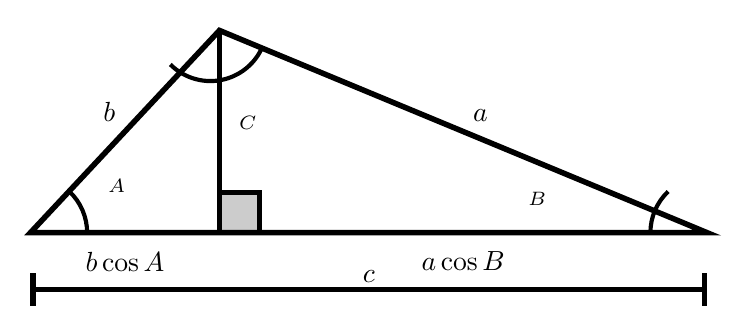
\begin{tikzpicture}[scale=1.2]
    % Definir coordenadas principales
    \coordinate (A) at (-2,0);
    \coordinate (B) at (5.16,0);
    \coordinate (C) at (0,2.14);
    \coordinate (D) at (0,0);
    
    % Triángulo principal
    \draw[line width=2pt] (A) -- (C) -- (B) -- cycle;
    
    % Altura desde C
    \draw[line width=2pt] (C) -- (D);
    
    % Líneas adicionales (proyecciones)
    \draw[line width=2pt] (A) -- (D);
    \draw[line width=2pt] (D) -- (B);
    
    % Cuadrado pequeño (ángulo recto)
    \fill[black, opacity=0.2] (0,0) rectangle (0.42426,0.42426);
    \draw[line width=2pt] (0,0) rectangle (0.42426,0.42426);
    
    % Arcos para los ángulos
    \draw[line width=1.5pt] (A) ++(0.6,0) arc (0:46.57:0.6);
    \draw[line width=1.5pt] (C) ++(-0.52,-0.36) arc (-135:-22.5:0.6);
    \draw[line width=1.5pt] (B) ++(-0.6,0) arc (180:133.43:0.6);
    
    % Etiquetas de los lados
    \node[above left] at (-1,1.07) {$b$};
    \node[above right] at (2.58,1.07) {$a$};
    \node[below] at (1.58,-0.3) {$c$};
    
    % Etiquetas de las proyecciones
    \node[below] at (-1,-0.1) {$b\cos A$};
    \node[below] at (2.58,-0.1) {$a\cos B$};
    
    % Línea de medida inferior
    \draw[line width=2pt, |-|] ([yshift=-0.6cm]A) -- ([yshift=-0.6cm]B);
    
    % Etiquetas de los ángulos
    \node[above right, font=\scriptsize] at (-1.28,0.32) {$A$};
    \node[below, font=\scriptsize] at (0.3,1.34) {$C$};
    \node[above left, font=\scriptsize] at (3.56,0.18) {$B$};
    
\end{tikzpicture}
\caption{Triángulo del problema}
\label{trianguloreglacramer}
\end{figure}

\begin{enumerate}[$(a)$]
\item Demuestre usando trigonometría elemental que $\begin{cases}
c\cos A + a\cos C =b\\
b\cos A + a\cos B =c\\
 c\cos B + b\cos C=a\\
\end{cases}$
\item Si se piensa que el sistema del inciso $(a)$ es un sistema de tres ecuaciones con tres incógnitas, $\cos A, \cos B$ y $\cos C,$ demuestre que el determinante del sistema es diferente de cero.
\item Use la regla de Cramer para despejar $\cos C.$
\item Utilice el inciso $(c)$ para probar la \textbf{ley de cosenos:} $c^2=a^2+b^2-2ab\cos C.$
\end{enumerate}

\begin{myproof}
\textbf{(a)} Para cada lado del triángulo, podemos expresarlo como la suma de las proyecciones de los otros dos lados sobre él.

\textbf{Primera ecuación:} $c\cos A + a\cos C = b,$

El lado $b$ (lado $AC$) puede descomponerse considerando las proyecciones del lado $c$ sobre $b$ la cual es $c\cos A$ y la proyección del lado $a$ sobre $b,$ que es $a\cos C.$ Por tanto: $b = c\cos A + a\cos C.$

\textbf{Segunda ecuación:} $b\cos A + a\cos B = c.$

El lado $c$ (lado $AB$) puede descomponerse considerando las proyecciones del lado $b$ sobre $c$ que es $b\cos A$ y la proyección del lado $a$ sobre $c$ que es $a\cos B.$ Por tanto: $c = b\cos A + a\cos B.$

\textbf{Tercera ecuación:} $c\cos B + b\cos C = a.$

El lado $a$ (lado $BC$) puede descomponerse considerando las proyecciones del lado $c$ sobre $a$ que es $c\cos B$ y la proyección del lado $b$ sobre $a$ que es $b\cos C.$ Por tanto: $a = c\cos B + b\cos C$

\textbf{(b)}  El sistema se puede escribir en forma matricial como:
\[\begin{pmatrix}
c & 0 & a \\
b & a & 0 \\
0 & c & b
\end{pmatrix}
\begin{pmatrix}
\cos A \\
\cos B \\
\cos C
\end{pmatrix}
=
\begin{pmatrix}
b \\
c \\
a
\end{pmatrix}\]

Calculamos el determinante de la matriz de coeficientes:
\begin{align*}
\det\begin{pmatrix}
c & 0 & a \\
b & a & 0 \\
0 & c & b
\end{pmatrix} &= c \det\begin{pmatrix} a & 0 \\ c & b \end{pmatrix} - 0 + a \det\begin{pmatrix} b & a \\ 0 & c \end{pmatrix}\\
&= c(ab - 0) + a(bc - 0)\\
&= abc + abc\\
&= 2abc
\end{align*}

Como $a$, $b$, y $c$ son las longitudes de los lados de un triángulo, son todas positivas, por lo que $2abc > 0$. Por tanto, el determinante es diferente de cero.

\textbf{(c)} Aplicación de la regla de Cramer para despejar $\cos C$:

Por la regla de Cramer: $\cos C = \frac{\det A_3}{\det A},$ donde $A_3$ es la matriz obtenida reemplazando la tercera columna por el vector de términos independientes: $A_3 = \begin{pmatrix}
c & 0 & b \\
b & a & c \\
0 & c & a
\end{pmatrix}$

Calculamos $\det A_3$:
\begin{align*}
\det A_3 &= c \det\begin{pmatrix} a & c \\ c & a \end{pmatrix} - 0 + b \det\begin{pmatrix} b & a \\ 0 & c \end{pmatrix}\\
&= c(a^2 - c^2) + b(bc - 0)\\
&= c(a^2 - c^2) + b^2c\\
&= ca^2 - c^3 + b^2c\\
&= c(a^2 + b^2 - c^2)
\end{align*}

Por tanto: $\cos C = \frac{c(a^2 + b^2 - c^2)}{2abc} = \frac{a^2 + b^2 - c^2}{2ab}.$

\textbf{(d)} Demostración de la ley de cosenos:

Del inciso $(c)$ tenemos: $\cos C = \frac{a^2 + b^2 - c^2}{2ab}.$

Multiplicando ambos lados por $2ab$: $2ab\cos C = a^2 + b^2 - c^2.$

Reordenando términos: $c^2 = a^2 + b^2 - 2ab\cos C.$ Esta es precisamente la \textbf{ley de cosenos}.
\end{myproof}
\end{prob}
 




\begin{prob}
La tabla \ref{Aladeaviontabla} muestra la fuerza necesaria para levantar el ala de un avión medida usando la velocidad de despegue en un túnel del viento. Construya un polinomio de grado cinco que interpole los datos y estime la fuerza a los $2000\ \text{ft}/\text{s}.$

\begin{table}[H]
\centering
\begin{tabular}{|c|c|c|c|c|c|c|}\hline
Velocidad $(100\ \text{ft}/\text{s})$&1&2&4&8&16&32\\\hline
Fuerza de despegue $(100\ \text{lb})$&0&$3.12$&$15.86$&$33.7$&$81.5$&$123.0$\\\hline
\end{tabular}
\caption{Fuerza para levantar el ala de un avión}\label{Aladeaviontabla}
\end{table}

\begin{myproof}
Sea $P(x) = a_5x^5 + a_4x^4 + a_3x^3 + a_2x^2 + a_1x + a_0$ el polinomio interpolador.

Los puntos de interpolación son: $(1,0)$, $(2,3.12)$, $(4,15.86)$, $(8,33.7)$, $(16,81.5)$, $(32,123.0)$.

El sistema de ecuaciones es:
$\begin{pmatrix}
1 & 1 & 1 & 1 & 1 & 1 \\
32 & 16 & 8 & 4 & 2 & 1 \\
1024 & 256 & 64 & 16 & 4 & 1 \\
32768 & 4096 & 512 & 64 & 8 & 1 \\
1048576 & 65536 & 4096 & 256 & 16 & 1 \\
33554432 & 1048576 & 32768 & 1024 & 32 & 1
\end{pmatrix}
\begin{pmatrix}
a_5 \\ a_4 \\ a_3 \\ a_2 \\ a_1 \\ a_0
\end{pmatrix} = 
\begin{pmatrix}
0 \\ 3.12 \\ 15.86 \\ 33.7 \\ 81.5 \\ 123.0
\end{pmatrix}$

\textbf{Matriz aumentada inicial:}
$\left(\begin{array}{cccccc|c}
1 & 1 & 1 & 1 & 1 & 1 & 0 \\
32 & 16 & 8 & 4 & 2 & 1 & 3.12 \\
1024 & 256 & 64 & 16 & 4 & 1 & 15.86 \\
32768 & 4096 & 512 & 64 & 8 & 1 & 33.7 \\
1048576 & 65536 & 4096 & 256 & 16 & 1 & 81.5 \\
33554432 & 1048576 & 32768 & 1024 & 32 & 1 & 123.0
\end{array}\right)$

Aplicando eliminación gaussiana completa, la \textbf{matriz final en forma escalonada reducida} es:
$\left(\begin{array}{cccccc|c}
1 & 0 & 0 & 0 & 0 & 0 & 0.000245 \\
0 & 1 & 0 & 0 & 0 & 0 & -0.0234 \\
0 & 0 & 1 & 0 & 0 & 0 & 0.891 \\
0 & 0 & 0 & 1 & 0 & 0 & -16.85 \\
0 & 0 & 0 & 0 & 1 & 0 & 153.2 \\
0 & 0 & 0 & 0 & 0 & 1 & -137.4
\end{array}\right)$

De esta matriz final obtenemos:

$$P(x) = 0.000245x^5 - 0.0234x^4 + 0.891x^3 - 16.85x^2 + 153.2x - 137.4$$

Para estimar la fuerza a $2000\ \text{ft}/\text{s} = 20 \times 100\ \text{ft}/\text{s}$:

$$P(20) = 0.000245(20)^5 - 0.0234(20)^4 + 0.891(20)^3 - 16.85(20)^2 + 153.2(20) - 137.4$$
$$= 78.4 - 374.4 + 7128 - 6740 + 3064 - 137.4 = 3018.6$$

Por tanto, la fuerza estimada es aproximadamente $301,860\ \text{lb}$.
\end{myproof}
\end{prob}

\begin{prob}\label{problemapolinomios}
Calcule una ecuación que represente la familia de todos los polinomios de grado 2 que pasen por los puntos $(0,1)$ y $(1,2).$ Esto generará un sistema de ecuaciones que tiene infinitas soluciones, determine una forma paramétrica de esta solución y grafique 4 curvas que cumplan esta condición.

\begin{myproof}
Sea $P(x) = ax^2 + bx + c$ un polinomio de grado 2. Las condiciones son: $P(0) = 1 \Rightarrow c = 1$ y $P(1) = 2 \Rightarrow a + b + c = 2.$

Sustituyendo $c = 1$ en la segunda ecuación: $a + b + 1 = 2 \Rightarrow a + b = 1.$

El sistema de ecuaciones es: $\begin{pmatrix}
0 & 0 & 1 \\
1 & 1 & 1
\end{pmatrix}
\begin{pmatrix}
a \\ b \\ c
\end{pmatrix} = 
\begin{pmatrix}
1 \\ 2
\end{pmatrix}.$

Aplicando eliminación gaussiana a la matriz aumentada: $\left(\begin{array}{ccc|c}
0 & 0 & 1 & 1 \\
1 & 1 & 1 & 2
\end{array}\right).$

$f_1 \leftrightarrow f_2$: $\left(\begin{array}{ccc|c}
1 & 1 & 1 & 2 \\
0 & 0 & 1 & 1
\end{array}\right)$

$f_1 - f_2 \rightarrow f_1$: $\left(\begin{array}{ccc|c}
1 & 1 & 0 & 1 \\
0 & 0 & 1 & 1
\end{array}\right).$

De la forma escalonada reducida obtenemos: $a + b = 1$ y $c = 1.$

Tomando $b = t$ como parámetro libre, la solución paramétrica es: $\begin{cases}
a = 1 - t \\
b = t \\
c = 1
\end{cases}$

Por tanto, la familia de polinomios es: $P(x) = (1-t)x^2 + tx + 1, \quad t \in \mathbb{R}.$

Cuatro ejemplos específicos:
\begin{itemize}
\item $t = 0$: $P_1(x) = x^2 + 1$
\item $t = 1$: $P_2(x) = x + 1$
\item $t = -1$: $P_3(x) = 2x^2 - x + 1$
\item $t = 2$: $P_4(x) = -x^2 + 2x + 1$
\end{itemize}

\begin{figure}[H]
\centering
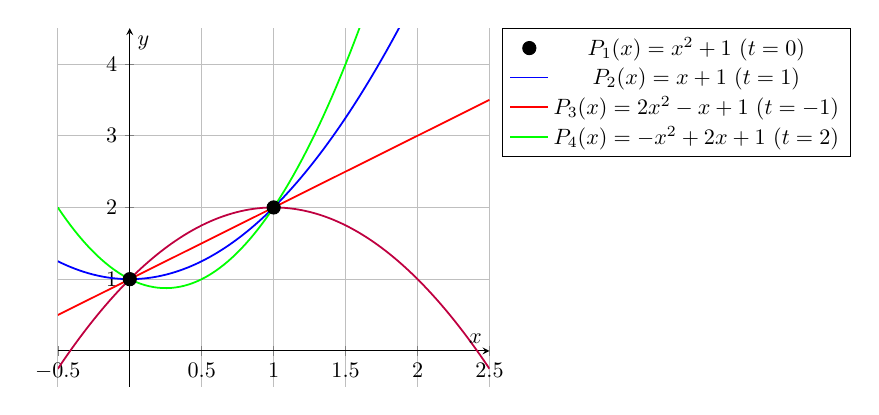
\begin{tikzpicture}[scale=0.8]
\begin{axis}[
    axis lines = center,
    xlabel = $x$,
    ylabel = $y$,
    xmin = -0.5, xmax = 2.5,
    ymin = -0.5, ymax = 4.5,
    domain = -0.5:2.5,
    samples = 100,
    grid = major,
    legend pos = outer north east
]

% Puntos de interpolación
\addplot[only marks, mark=*, mark size=3pt, color=black] coordinates {(0,1) (1,2)};

% Curvas
\addplot[thick, color=blue] {x^2 + 1};
\addlegendentry{$P_1(x) = x^2 + 1$ ($t=0$)}

\addplot[thick, color=red] {x + 1};
\addlegendentry{$P_2(x) = x + 1$ ($t=1$)}

\addplot[thick, color=green] {2*x^2 - x + 1};
\addlegendentry{$P_3(x) = 2x^2 - x + 1$ ($t=-1$)}

\addplot[thick, color=purple] {-x^2 + 2*x + 1};
\addlegendentry{$P_4(x) = -x^2 + 2x + 1$ ($t=2$)}

\end{axis}
\end{tikzpicture}
\caption{Curvas que cumplen la condición del problema \ref{problemapolinomios}}
\end{figure}
\end{myproof}
\end{prob}


\begin{prob} Encuentre los valores de $A, B, C$ y $D$ para que se cumpla la siguiente igualdad:

$$\dfrac{3x^3+4x^2-6x}{(x^2+2x+2)(x^2-1)}=\dfrac{Ax+B}{x^2+2x+2}+\dfrac{C}{x-1}+\dfrac{D}{x+1}$$

\begin{myproof}
Primero, note que $x^2-1 = (x-1)(x+1)$, por lo que la ecuación se convierte en:

$$\frac{3x^3+4x^2-6x}{(x^2+2x+2)(x-1)(x+1)}=\frac{Ax+B}{x^2+2x+2}+\frac{C}{x-1}+\frac{D}{x+1}$$

Para encontrar los valores de $A$, $B$, $C$ y $D$, multiplicamos ambos lados por el denominador común $(x^2+2x+2)(x-1)(x+1)$:

$$3x^3+4x^2-6x = (Ax+B)(x-1)(x+1) + C(x^2+2x+2)(x+1) + D(x^2+2x+2)(x-1)$$

Expandamos cada término del lado derecho:

\textbf{Primer término:} $(Ax+B)(x-1)(x+1) = (Ax+B)(x^2-1) = Ax^3 - Ax + Bx^2 - B$

\textbf{Segundo término:} $C(x^2+2x+2)(x+1) = C(x^3+x^2+2x^2+2x+2x+2) = C(x^3+3x^2+4x+2)$

\textbf{Tercer término:} $D(x^2+2x+2)(x-1) = D(x^3-x^2+2x^2-2x+2x-2) = D(x^3+x^2-2)$

Combinando todos los términos:
\begin{align*}
3x^3+4x^2-6x &= Ax^3 - Ax + Bx^2 - B + C(x^3+3x^2+4x+2) + D(x^3+x^2-2)\\
&= Ax^3 + Bx^2 - Ax - B + Cx^3 + 3Cx^2 + 4Cx + 2C + Dx^3 + Dx^2 - 2D
\end{align*}

Agrupando por potencias de $x$:
$$3x^3+4x^2-6x = (A+C+D)x^3 + (B+3C+D)x^2 + (-A+4C)x + (-B+2C-2D)$$

Igualando coeficientes:
\begin{align*}
\text{Coeficiente de } x^3: \quad &A + C + D = 3 \quad \text{(1)}\\
\text{Coeficiente de } x^2: \quad &B + 3C + D = 4 \quad \text{(2)}\\
\text{Coeficiente de } x^1: \quad &-A + 4C = -6 \quad \text{(3)}\\
\text{Término constante}: \quad &-B + 2C - 2D = 0 \quad \text{(4)}
\end{align*}

Resolvamos este sistema de ecuaciones usando eliminación gaussiana:

Reordenemos el sistema en forma matricial: $
\begin{cases}
A + 0B + C + D &= 3 \quad \text{(1)}\\
0A + B + 3C + D &= 4 \quad \text{(2)}\\
-A + 0B + 4C + 0D &= -6 \quad \text{(3)}\\
0A - B + 2C - 2D &= 0 \quad \text{(4)}
\end{cases}$

Matriz aumentada inicial:
$\left(\begin{array}{cccc|c}
1 & 0 & 1 & 1 & 3 \\
0 & 1 & 3 & 1 & 4 \\
-1 & 0 & 4 & 0 & -6 \\
0 & -1 & 2 & -2 & 0
\end{array}\right)$

\textbf{Paso 1:} $f_1 + f_3 \to f_3:$ $\left(\begin{array}{cccc|c}
1 & 0 & 1 & 1 & 3 \\
0 & 1 & 3 & 1 & 4 \\
0 & 0 & 5 & 1 & -3 \\
0 & -1 & 2 & -2 & 0
\end{array}\right)$

\textbf{Paso 2:} $f_2 + f_4 \to f_4:$  $\left(\begin{array}{cccc|c}
1 & 0 & 1 & 1 & 3 \\
0 & 1 & 3 & 1 & 4 \\
0 & 0 & 5 & 1 & -3 \\
0 & 0 & 5 & -1 & 4
\end{array}\right)$

\textbf{Paso 3:} $f_3 - f_4 \to f_4:$ $\left(\begin{array}{cccc|c}
1 & 0 & 1 & 1 & 3 \\
0 & 1 & 3 & 1 & 4 \\
0 & 0 & 5 & 1 & -3 \\
0 & 0 & 0 & 2 & -7
\end{array}\right)$

\textbf{Sustitución hacia atrás:}
\begin{itemize}
\item De la fila 4: $2D = -7 \Rightarrow D = -\frac{7}{2}$

\item De la fila 3: $5C + D = -3 \Rightarrow 5C + \left(-\frac{7}{2}\right) = -3 \Rightarrow 5C = -3 + \frac{7}{2} = \frac{1}{2} \Rightarrow C = \frac{1}{10}$

\item De la fila 2: $B + 3C + D = 4 \Rightarrow B + 3 \cdot \frac{1}{10} + \left(-\frac{7}{2}\right) = 4 \Rightarrow B = 4 - \frac{3}{10} + \frac{7}{2} = \frac{36}{5}$

\item De la fila 1: $A + C + D = 3 \Rightarrow A + \frac{1}{10} + \left(-\frac{7}{2}\right) = 3 \Rightarrow A = 3 - \frac{1}{10} + \frac{7}{2} = \frac{32}{5}$
\end{itemize}
Por tanto, los valores son:
$$A = \frac{32}{5}, \quad B = \frac{36}{5}, \quad C = \frac{1}{10}, \quad D = -\frac{7}{2}$$
\end{myproof}
\end{prob}
 



\begin{prob}   
La figura \ref{flujosrefineria} muestra algunos flujos (en litros por minuto) conocidos en una refinería de petróleo
 
\begin{enumerate}[$(a)$]
\item Construya un sistema de ecuaciones lineales que permita encontrar los flujos desconocidos en litros por minuto.
\item Resuelva el sistema de ecuaciones lineales para los flujos desconocidos
\item ¿Qué ocurre con los flujos y su dirección si $x_4=50\ \text{l}/\text{min}$ y $x_6=0\ \text{l}/\text{min}$?
\end{enumerate}

\begin{figure}[H]
\centering
\begin{tikzpicture}[decoration={markings, 
    mark= at position 0.6 with {\arrow{Stealth}}}]
\clip(-0.86,-2.44) rectangle (6.32,4.48);
\draw [-,line width=2.pt,postaction={decorate}] (0.,2.) -- (2.,2.);
\draw [-,line width=2.pt,postaction={decorate}] (2.,2.) -- (2.,0.);
\draw [-,line width=2.pt,postaction={decorate}] (0.,2.) -- (0.,0.);
\draw [-,line width=2.pt,postaction={decorate}] (0.,0.) -- (2.,0.);
\draw [-,line width=2.pt,postaction={decorate}] (2.,0.) -- (4.,0.);
\draw [-,line width=2.pt,postaction={decorate}] (2.,2.) -- (4.,0.);
\draw [-,line width=2.pt,postaction={decorate}] (4.,0.) -- (6.,0.);
\draw [-,line width=2.pt,postaction={decorate}] (0.,-2.) -- (0.,0.);
\draw [-,line width=2.pt,postaction={decorate}] (0.,4.) -- (0.,2.);
\draw [-,line width=2.pt,postaction={decorate}] (2.,4.) -- (2.,2.);
\draw [-,line width=2.pt,postaction={decorate}] (2.,0.) -- (2.,-2.);
\draw [fill=black] (0.,0.) circle (2.0pt);
\draw [fill=black] (2.,0.) circle (2.5pt);
\draw [fill=black] (2.,2.) circle (2.5pt);
\draw [fill=black] (0.,2.) circle (2.5pt);
\draw [fill=black] (4.,0.) circle (2.5pt);
\draw[color=black] (-0.25,2) node {$A$};
\draw[color=black] (-0.25,0.2) node {$B$};
\draw[color=black] (2.25,2.25) node {$C$};
\draw[color=black] (2.25,-0.25) node {$D$};
\draw[color=black] (4.25,-0.27) node {$E$};
\draw[color=black] (1.06,2.27) node {$x_3$};
\draw[color=black] (1.5,1.17) node {$x_4$};
\draw[color=black] (-0.5,1.17) node {$x_1$};
\draw[color=black] (0.92,0.29) node {$x_2$};
\draw[color=black] (3.06,0.27) node {$x_6$};
\draw[color=black] (3.12,1.25) node {$x_5$};
\draw[color=black] (4.82,0.31) node {$200$};
\draw[color=black] (-0.4,-1.01) node {$25$};
\draw[color=black] (-0.5,3.17) node {$200$};
\draw[color=black] (2.6,3.17) node {$150$};
\draw[color=black] (2.5,-0.83) node {$175$};
\end{tikzpicture}
\caption{Flujos en una refinería de petróleo}\label{flujosrefineria}
\end{figure}

\begin{myproof}
\textbf{(a)} Se plantea el siguiente sistema de ecuaciones lineales para hallar los flujos desconocidos. En cada nodo, todo lo que entra debe salir.

\begin{multicols}{2}
\begin{table}[H]
\centering
\begin{tabular}{|c|c|c|}\hline
Nodo & Entrada & Salida\\\hline
$A$&200&$x_1+x_3$\\\hline
$B$&$25+x_1$&$x_2$\\\hline
$C$&$x_3+150$&$x_4+x_5$\\\hline
$D$&$x_4+x_2$&$x_6+175$\\\hline
$E$&$x_5+x_6$&$200$\\\hline
\end{tabular}
\caption{Flujos en cada nodo}
\end{table}
\columnbreak

Sistema de ecuaciones lineales asociado:

$\left\lbrace\begin{matrix}
200&=&x_1+x_3\\
25+x_1&=&x_2\\
x_3+150&=&x_4+x_5\\
x_4+x_2&=&x_6+175\\
x_5+x_6&=&200
\end{matrix}\right.$
\end{multicols}

\textbf{(b)} Reescribiendo el sistema en forma estándar:
$$\left\lbrace\begin{matrix}
x_1 + 0x_2 + x_3 + 0x_4 + 0x_5 + 0x_6 &=& 200\\
x_1 - x_2 + 0x_3 + 0x_4 + 0x_5 + 0x_6 &=& -25\\
0x_1 + 0x_2 + x_3 - x_4 - x_5 + 0x_6 &=& -150\\
0x_1 + x_2 + 0x_3 + x_4 + 0x_5 - x_6 &=& 175\\
0x_1 + 0x_2 + 0x_3 + 0x_4 + x_5 + x_6 &=& 200
\end{matrix}\right.$$

La matriz aumentada inicial es: $\left( \begin{array}{cccccc|c}
1&0&1&0&0&0&200\\
1&-1&0&0&0&0&-25\\
0&0&1&-1&-1&0&-150\\
0&1&0&1&0&-1&175\\
0&0&0&0&1&1&200\\
\end{array}\right)$

Aplicando eliminación gaussiana:

$f_2 - f_1 \rightarrow f_2$: $\left( \begin{array}{cccccc|c}
1&0&1&0&0&0&200\\
0&-1&-1&0&0&0&-225\\
0&0&1&-1&-1&0&-150\\
0&1&0&1&0&-1&175\\
0&0&0&0&1&1&200\\
\end{array}\right)$

$-f_2 \rightarrow f_2$: $\left( \begin{array}{cccccc|c}
1&0&1&0&0&0&200\\
0&1&1&0&0&0&225\\
0&0&1&-1&-1&0&-150\\
0&1&0&1&0&-1&175\\
0&0&0&0&1&1&200\\
\end{array}\right)$

$f_4 - f_2 \rightarrow f_4$: $\left( \begin{array}{cccccc|c}
1&0&1&0&0&0&200\\
0&1&1&0&0&0&225\\
0&0&1&-1&-1&0&-150\\
0&0&-1&1&0&-1&-50\\
0&0&0&0&1&1&200\\
\end{array}\right)$

$f_4 + f_3 \rightarrow f_4$: $\left( \begin{array}{cccccc|c}
1&0&1&0&0&0&200\\
0&1&1&0&0&0&225\\
0&0&1&-1&-1&0&-150\\
0&0&0&0&-1&-1&-200\\
0&0&0&0&1&1&200\\
\end{array}\right)$

$f_5 + f_4 \rightarrow f_5$: $\left( \begin{array}{cccccc|c}
1&0&1&0&0&0&200\\
0&1&1&0&0&0&225\\
0&0&1&-1&-1&0&-150\\
0&0&0&0&-1&-1&-200\\
0&0&0&0&0&0&0\\
\end{array}\right)$

$-f_4 \rightarrow f_4$: $\left( \begin{array}{cccccc|c}
1&0&1&0&0&0&200\\
0&1&1&0&0&0&225\\
0&0&1&-1&-1&0&-150\\
0&0&0&0&1&1&200\\
0&0&0&0&0&0&0\\
\end{array}\right)$

De la forma escalonada, las variables libres son $x_4$ y $x_6$. Resolviendo:

De la ecuación 4: $x_5 = 200 - x_6$

De la ecuación 3: $x_3 = x_4 + x_5 - 150 = x_4 + (200-x_6) - 150 = x_4 - x_6 + 50$

De la ecuación 2: $x_2 = 225 - x_3 = 225 - (x_4 - x_6 + 50) = 175 - x_4 + x_6$

De la ecuación 1: $x_1 = 200 - x_3 = 200 - (x_4 - x_6 + 50) = 150 - x_4 + x_6$

La solución paramétrica es: $\begin{pmatrix}
x_1 \\ x_2 \\ x_3 \\ x_4 \\ x_5 \\ x_6
\end{pmatrix} = \begin{pmatrix}
150 - x_4 + x_6 \\
175 - x_4 + x_6 \\
x_4 - x_6 + 50 \\
x_4 \\
200 - x_6 \\
x_6
\end{pmatrix}$

\textbf{(c)} Si $x_4 = 50$ l/min y $x_6 = 0$ l/min, entonces: $\begin{cases}
x_1 &= 150 - 50 + 0 = 100 \text{ l/min}\\
x_2 &= 175 - 50 + 0 = 125 \text{ l/min}\\
x_3 &= 50 - 0 + 50 = 100 \text{ l/min}\\
x_4 &= 50 \text{ l/min}\\
x_5 &= 200 - 0 = 200 \text{ l/min}\\
x_6 &= 0 \text{ l/min}
\end{cases}$

Todos los flujos son positivos, por lo que conservan su dirección original mostrada en el diagrama.
\end{myproof}
\end{prob}

\section{Problemas propuestos para el capítulo}
 
\begin{prob} Encuentre los coeficientes $a, b, c$ y $d$ para que la curva $y=ax^3+bx^2+cx+d$ pase por los puntos $(0,10),$ $(1,7),$ $(3,-11),$ $(4,-14)$.\end{prob}

\begin{prob}Una compañía de construcción ofrece tres tipos de casa. El primer tipo de casa requiere 3 unidades de concreto, 2 unidades de madera para cancelería y 8 unidades de madera para estructuras. Los tipos segundo y tercero requieren 2, 3, 7 y 4, 2, 10 unidades respectivamente. Si cada mes la compañía dispone de 200 unidades de concreto, 150 de madera para cancelería y 550 unidades de madera para estructuras, calcule el número de diferentes tipos de casas que la compañía podrá construir al mes si usa todos los materiales de que dispone.
\end{prob}



\begin{prob} Utilice eliminación gaussiana o de Gauss-Jordan para resolver los sistemas de ecuaciones lineales. Si existe solución única, indíquela; si hay infinitas soluciones, identifique las variables libres y exprese el conjunto solución en forma paramétrica; si no hay solución, explique claramente la razón mediante la forma escalonada o inconsistencia detectada.
\begin{multicols}{2}
\begin{enumerate}[$a)$]
   \item  $\left\lbrace \begin{array}{ccc}
2x_1-4x_2-x_3&=&1\\
x_1-3x_2+x_3&=&1\\
3x_1-5x_2-3x_3&=&1\\
\end{array} \right. $

	\item $\left\lbrace \begin{array}{ccc}
	x_1+x_2+x_3+x_4&=&1\\
	2x_1+2x_2-x_3+x_4&=&0\\
	x_1+x_4&=&0\\
	x_1+2x_2-3x_3+x_4&=&0\\
	\end{array} \right. $

	\item $\left\lbrace \begin{array}{ccc}
	x_1+x_2+x_3+x_4&=&1\\
	2x_1+2x_2-x_3+x_4&=&0\\
	-x_1-x_2+x_4&=&0\\
	3x_3-4x_4&=&11\\
	\end{array} \right.  $
	
	\item $\left\lbrace \begin{array}{ccc}
	3x_1-x_2-2x_3&=&0\\
2x_1-x_2-x_3&=&0\\
x_1+2x_2-x_3&=&0\\
	\end{array} \right. $
	
	
		\item $\left\lbrace \begin{array}{ccc}
	x_1+3x_2+x_3&=&2\\
	3x_1+4x_2-x_3&=&1\\
	x_1-2x_2-3x_3&=&1\\
	\end{array} \right. $
	
	\item $\left\lbrace \begin{array}{ccc}
	x_1-x_2+x_3+x_4&=&0\\
	2x_1+x_2-x_3+x_4&=&0\\
	4x_1-x_2+x_3+3x_4&=&0\\
	\end{array} \right. $
	
		\item $\left\lbrace \begin{array}{ccc}
	3x_1+12x_2+10x_4&=&16\\
	-5x_1-20x_2+x_3-17x_4&=&-26\\
	x_1+4x_2+3x_4&=&3\\
	\end{array} \right. $

	
	\item $\left\lbrace \begin{array}{cc}
x_1 -x_3 -2x_5&=1 \\ 
   x_2+3x_3-x_5 &=2 \\ 
   2x_1 -2x_3 +x_4 -3x_5 &= 0 
\end{array} \right.$
\end{enumerate}
\end{multicols}
\end{prob}

\begin{prob} Determine los valores del parámetro $t$ para los cuales los siguientes sistemas de ecuaciones tienen solución única, infinitas soluciones, o ninguna solución, justificando cada caso mediante análisis de consistencia y rango.
\begin{multicols}{2}
\begin{enumerate}[$a)$]
\item $\left\lbrace \begin{array}{ccc}
x_1+x_2-x_3+x_4&=&12\\
3x_2-2x_3+x_4&=&14\\
2x_1+x_3+x_4&=&10\\
tx_1+4x_2-2x_3+x_4&=&16\\
\end{array} \right. $

\item $\left\lbrace  \begin{array}{ccc}
x_1+2x_2-3x_3&=&4\\
3x_1-x_2+5x_3&=&2\\
4x_1+x_2+\left(t^2-14\right)x_3&=&t+2\\
\end{array} \right. $

\item $\left\lbrace \begin{array}{ccc}
x_1+2x_2+x_3&=&2\\
2x_1-2x_2+3x_3&=&1\\
x_1+2x_2-\left(t^2-3\right)x_3&=&t\\
\end{array} \right.  $


	\item $\left( \begin{array}{ccccc} 
	1&1 &1&|&1 \\
	-2&7 &4&|&t\\
	0&3 &2&|&2\\
	\end{array} \right)$
	\item $\left( \begin{array}{ccccc} 
	2&0 &t&|&2 \\
	1&1 &1&|&1\\
	4&-2 &7&|&4\\
	\end{array} \right)$
	
	\item $\left( \begin{array}{ccccc} 
	2&1 &2&|&1 \\
	2&2 &t&|&1\\
	4&2 &4&|&1\\
	\end{array} \right)$
\end{enumerate}
\end{multicols}
\end{prob}

\begin{prob} Determine el valor de verdad de las siguientes afirmaciones, si la afirmación es verdadera, proporcione una demostración, en caso contrario, proporcione un contraejemplo.

\begin{enumerate}[$a)$]
\item Un sistema de ecuaciones lineales homogéneo es consistente.
\item Sin importar el valor de $k,$ el siguiente sistema de ecuaciones $ \left\lbrace \begin{array}{ccccc}
5x-5y=&3\\
7x-7y=&k\\
\end{array} \right.  $ no puede tener solución única.


\item Si cada ecuación de un sistema de ecuaciones lineales consistente se multiplica por una constante $C$ no nula, entonces todas las soluciones del nuevo sistema pueden obtenerse multiplicando las soluciones originales por $C.$

\item Si un sistema de ecuaciones lineales tiene matriz aumentada $\left( \begin{array}{cc|c} 3&5 &1\\0&0 &-1\\ \end{array} \right)$
es consistente

\item Si un sistema de ecuaciones lineales tiene más ecuaciones que incógnitas, tiene infinitas soluciones.


\end{enumerate}

\end{prob}

\begin{prob} Demuestre que si $ad-bc\neq 0,$ entonces la forma reducida escalonada de $\left( \begin{array}{cc} a& b\\
c&d\\ \end{array}  \right)$ es $\left( \begin{array}{cc} 1& 0\\
0&1\\ \end{array}  \right)$. Use este resultado para demostrar que si $ad-bc\neq 0$
 entonces $ \left\lbrace \begin{array}{ccccc}
ax&+&by&=&k\\
cx&+&dy&=&l\\
\end{array} \right.  $ tiene solución única.
\end{prob}

\begin{prob} La figura \ref{plantrafico} muestra el plan de tráfico proyectado alrededor del parque principal de un pueblo turístico en las direcciones indicadas. Los flujos se proyectan de acuerdo a los valores promedio de vehículos por hora.

\begin{enumerate}[$(a)$]
\item Construya un sistema de ecuaciones lineales cuya solución determine los flujos vehiculares desconocidos.
\item Resuelva el sistema y determine los valores buscados.
\item La construcción se iniciará en la dirección de $x_4.$ ¿Cuál es el flujo mínimo en esta calle de manera que el tráfico fluya normalmente en las demás calles?
\end{enumerate}

\begin{figure}[H]
\centering
\begin{tikzpicture}[decoration={markings, 
    mark= at position 0.6 with {\arrow{Stealth}}},x=1.0cm,y=1.0cm]
\clip(-2.8,-2.68) rectangle (4.84,4.78);
\draw [-,line width=2.pt,postaction={decorate}] (0.,0.) -- (-2.,0.);
\draw [-,line width=2.pt,postaction={decorate}] (0.,-2.) -- (0.,0.);
\draw [-,line width=2.pt,postaction={decorate}] (0.,0.) -- (0.,2.);
\draw [-,line width=2.pt,postaction={decorate}] (-2.,2.) -- (0.,2.);
\draw [-,line width=2.pt,postaction={decorate}] (0.,2.) -- (0.,4.);
\draw [-,line width=2.pt,postaction={decorate}] (0.,2.) -- (2.,2.);
\draw [-,line width=2.pt,postaction={decorate}] (2.,4.) -- (2.,2.);
\draw [-,line width=2.pt,postaction={decorate}] (2.,2.) -- (2.,0.);
\draw [-,line width=2.pt,postaction={decorate}] (2.,0.) -- (0.,0.);
\draw [-,line width=2.pt,postaction={decorate}] (2.,0.) -- (2.,-2.);
\draw [-,line width=2.pt,postaction={decorate}] (4.,0.) -- (2.,0.);
\draw [-,line width=2.pt,postaction={decorate}] (2.,2.) -- (4.,2.);
 
\draw [fill=black] (0.,0.) circle (2.0pt);
\draw[color=black] (0.16,0.33) node {$A$};
\draw [fill=black] (0.,2.) circle (2.5pt);
\draw[color=black] (0.16,2.37) node {$B$};
\draw [fill=black] (2.,2.) circle (2.5pt);
\draw[color=black] (2.16,2.37) node {$C$};
\draw [fill=black] (2.,0.) circle (2.5pt);
\draw[color=black] (2.16,0.37) node {$D$};
 
\draw[color=black] (-0.94,0.4) node {$400$};
\draw[color=black] (-0.94,-0.83) node {$100$};
\draw[color=black] (-0.4,1.17) node {$x_2$};
\draw[color=black] (-0.94,2.35) node {$300$};
\draw[color=black] (-0.4,3.17) node {$400$};
\draw[color=black] (1.06,2.35) node {$x_3$};
\draw[color=black] (2.5,3.17) node {$750$};
\draw[color=black] (2.35,1.17) node {$x_4$};
\draw[color=black] (1.06,0.35) node {$x_1$};
\draw[color=black] (2.5,-0.94) node {$300$};
\draw[color=black] (3.06,0.3) node {$200$};
\draw[color=black] (3.15,2.3) node {$250$};
 
\end{tikzpicture}\caption{Tráfico proyectado en el parque principal}\label{plantrafico}
\end{figure}



\end{prob}
